%% TeX source for "Micrometeoroid events in LISA Pathfinder" 
%% Author: I. Thorpe, NASA/GSFC
%% Note: Compiled using AASTeX 6.2

\documentclass[twocolumn, trackchanges]{aastex62}
%% options are:
%%  twocolumn   : two text columns, 10 point font, single spaced article.
%%                This is the most compact and represent the final published
%%                derived PDF copy of the accepted manuscript from the publisher
%%  manuscript  : one text column, 12 point font, double spaced article.
%%  preprint    : one text column, 12 point font, single spaced article.  
%%  preprint2   : two text columns, 12 point font, single spaced article.
%%  modern      : a stylish, single text column, 12 point font, article with
%% 		  wider left and right margins. This uses the Daniel
%% 		  Foreman-Mackey and David Hogg design.
%%
%% Note that you can submit to the AAS Journals in any of these 6 styles.
%%
%% There are other optional arguments one can envoke to allow other stylistic
%% actions. The available options are:
%%
%%  astrosymb    : Loads Astrosymb font and define \astrocommands. 
%%  tighten      : Makes baselineskip slightly smaller, only works with 
%%                 the twocolumn substyle.
%%  times        : uses times font instead of the default
%%  linenumbers  : turn on lineno package.
%%  trackchanges : required to see the revision mark up and print its output
%%  longauthor   : Do not use the more compressed footnote style (default) for 
%%                 the author/collaboration/affiliations. Instead print all
%%                 affiliation information after each name. Creates a much
%%                 long author list but may be desirable for short author papers
%%
%% these can be used in any combination, e.g.
%%

%% Additional Packages
\usepackage{color}
\usepackage{amsmath} 
\usepackage{graphicx}

%% MACROs
\newcommand{\nwip}[2]{\langle #1|#2\rangle} % noise weighted inner product
\newcommand{\vdag}{(v)^\dagger}
\newcommand\aastex{AAS\TeX}
\newcommand\latex{La\TeX}
\newcommand{\red}[1]{\textcolor{red}{#1}}
\newcommand{\blue}[1]{\textcolor{blue}{#1}}
\newcommand{\nhits}{54 } % macro to keep number of impacts the same everywhere
\newcommand{\nhours}{4348 }

%data analysis variables
\newcommand{\data}{\tilde d}
\newcommand{\model}{\tilde h}
\newcommand{\residual}{\tilde r}
\newcommand{\params}{{\vec \lambda}}
\newcommand{\n}{\tilde n}
\newcommand{\Cij}{C_{ij}}
\newcommand{\Cii}{C_{ii}}
\newcommand{\invCij}{C_{ij}^{-1}}

%geometry 
\newcommand{\rcom}{{\bm r}^{C}} %center of mass w.r.t. body frame
\newcommand{\rgrs}{{\bm r}^{G}} %GRS w.r.t. body frame
\newcommand{\rth}[1]{{\bm r}^{#1}} %Thruster location w.r.t. body frame 
\newcommand{\rimp}{\bm r} %impact location w.r.t. body frame
\newcommand{\ehat}[1]{\hat{\bm e}^{#1}} %Thruster location w.r.t. body frame 
\newcommand{\I}{\bm I} %moment of inertia

%shortucts
\newcommand{\lin}{\bm x}
\newcommand{\ang}{\bm \omega}
\newcommand{\hvec}{\bm h}

%% Dates
\received{\today}
\revised{\today}
\accepted{\today}
%% Command to document which AAS Journal the manuscript was submitted to.
%% Adds "Submitted to " the arguement.
\submitjournal{ApJ}

%% Mark up commands to limit the number of authors on the front page.
%% Note that in AASTeX v6.1 a \collaboration call (see below) counts as
%% an author in this case.
%
%\AuthorCollaborationLimit=7
%
%% Will only show Schwarz, Muench and "the AAS Journals Data Scientist 
%% collaboration" on the front page of this example manuscript.
%%
%% Note that all of the author will be shown in the published article.
%% This feature is meant to be used prior to acceptance to make the
%% front end of a long author article more manageable. Please do not use
%% this functionality for manuscripts with less than 20 authors. Conversely,
%% please do use this when the number of authors exceeds 40.
%%
%% Use \allauthors at the manuscript end to show the full author list.
%% This command should only be used with \AuthorCollaborationLimit is used.

%% The following command can be used to set the latex table counters.  It
%% is needed in this document because it uses a mix of latex tabular and
%% AASTeX deluxetables.  In general it should not be needed.
%\setcounter{table}{1}

%%%%%%%%%%%%%%%%%%%%%%%%%%%%%%%%%%%%%%%%%%%%%%%%%%%%%%%%%%%%%%%%%%%%%%%%%%%%%%%%
%%
%% The following section outlines numerous optional output that
%% can be displayed in the front matter or as running meta-data.
%%
%% If you wish, you may supply running head information, although
%% this information may be modified by the editorial offices.
\shorttitle{Micrometeoroid Impacts in LISA Pathfinder}
\shortauthors{Thorpe, et al.}
%%
%% You can add a light gray and diagonal water-mark to the first page 
%% with this command:
% \watermark{text}
%% where "text", e.g. DRAFT, is the text to appear.  If the text is 
%% long you can control the water-mark size with:
%  \setwatermarkfontsize{dimension}
%% where dimension is any recognized LaTeX dimension, e.g. pt, in, etc.
%%
%%%%%%%%%%%%%%%%%%%%%%%%%%%%%%%%%%%%%%%%%%%%%%%%%%%%%%%%%%%%%%%%%%%%%%%%%%%%%%%%

%% This is the end of the preamble.  Indicate the beginning of the
%% manuscript itself with \begin{document}.

\begin{document}

\title{Micrometeoroid Events in LISA Pathfinder}

%% LaTeX will automatically break titles if they run longer than
%% one line. However, you may use \\ to force a line break if
%% you desire. In v6.1 you can include a footnote in the title.

%% A significant change from earlier AASTEX versions is in the structure for 
%% calling author and affilations. The change was necessary to implement 
%% autoindexing of affilations which prior was a manual process that could 
%% easily be tedious in large author manuscripts.
%%
%% The \author command is the same as before except it now takes an optional
%% arguement which is the 16 digit ORCID. The syntax is:
%% \author[xxxx-xxxx-xxxx-xxxx]{Author Name}
%%
%% This will hyperlink the author name to the author's ORCID page. Note that
%% during compilation, LaTeX will do some limited checking of the format of
%% the ID to make sure it is valid.
%%
%% Use \affiliation for affiliation information. The old \affil is now aliased
%% to \affiliation. AASTeX v6.1 will automatically index these in the header.
%% When a duplicate is found its index will be the same as its previous entry.
%%
%% Note that \altaffilmark and \altaffiltext have been removed and thus 
%% can not be used to document secondary affiliations. If they are used latex
%% will issue a specific error message and quit. Please use multiple 
%% \affiliation calls for to document more than one affiliation.
%%
%% The new \altaffiliation can be used to indicate some secondary information
%% such as fellowships. This command produces a non-numeric footnote that is
%% set away from the numeric \affiliation footnotes.  NOTE that if an
%% \altaffiliation command is used it must come BEFORE the \affiliation call,
%% right after the \author command, in order to place the footnotes in
%% the proper location.
%%
%% Use \email to set provide email addresses. Each \email will appear on its
%% own line so you can put multiple email address in one \email call. A new
%% \correspondingauthor command is available in V6.1 to identify the
%% corresponding author of the manuscript. It is the author's responsibility
%% to make sure this name is also in the author list.
%%
%% While authors can be grouped inside the same \author and \affiliation
%% commands it is better to have a single author for each. This allows for
%% one to exploit all the new benefits and should make book-keeping easier.
%%
%% If done correctly the peer review system will be able to
%% automatically put the author and affiliation information from the manuscript
%% and save the corresponding author the trouble of entering it by hand.

%% Define the addresses (at least for the LPF collaboration)

\def\addressa{European Space Astronomy Centre, European Space Agency, Villanueva de la
Ca\~{n}ada, 28692 Madrid, Spain}
\def\addressb{Albert-Einstein-Institut, Max-Planck-Institut f\"ur Gravitationsphysik und Leibniz Universit\"at Hannover,
Callinstra{\ss}e 38, 30167 Hannover, Germany}
\def\addressc{APC, Univ Paris Diderot, CNRS/IN2P3, CEA/lrfu, Obs de Paris, Sorbonne Paris Cit\'e, France}
\def\addressd{High Energy Physics Group, Physics Department, Imperial College London, Blackett Laboratory, Prince Consort Road, London, SW7 2BW, UK }
\def\addresse{Dipartimento di Fisica, Universit\`a di Roma ``Tor Vergata'',  and INFN, sezione Roma Tor Vergata, I-00133 Roma, Italy}
\def\addressf{Department of Industrial Engineering, University of Trento, via Sommarive 9, 38123 Trento, 
and Trento Institute for Fundamental Physics and Application / INFN}
\def\addressg{Airbus Defence and Space, Claude-Dornier-Strasse, 88090 Immenstaad, Germany}
\def\addressh{European Space Technology Centre, European Space Agency, 
Keplerlaan 1, 2200 AG Noordwijk, The Netherlands}
\def\addressi{Dipartimento di Fisica, Universit\`a di Trento and Trento Institute for 
Fundamental Physics and Application / INFN, 38123 Povo, Trento, Italy}
\def\addressj{The School of Physics and Astronomy, University of
Birmingham, Birmingham, UK}
\def\addressk{Airbus Defence and Space, Gunnels Wood Road, Stevenage, Hertfordshire, SG1 2AS, UK }
\def\addressl{Institut f\"ur Geophysik, ETH Z\"urich, Sonneggstrasse 5, CH-8092, Z\"urich, Switzerland}
\def\addressm{The UK Astronomy Technology Centre, Royal Observatory, Edinburgh, Blackford Hill, Edinburgh, EH9 3HJ, UK}
\def\addressn{Institut de Ci\`encies de l'Espai (CSIC-IEEC), Campus UAB, Carrer de Can Magrans s/n, 08193 Cerdanyola del Vall\`es, Spain}
\def\addresso{DISPEA, Universit\`a di Urbino ``Carlo Bo'', Via S. Chiara, 27 61029 Urbino/INFN, Italy}
\def\addressp{European Space Operations Centre, European Space Agency, 64293 Darmstadt, Germany }
\def\addressq{Physik Institut, 
Universit\"at Z\"urich, Winterthurerstrasse 190, CH-8057 Z\"urich, Switzerland}
\def\addressr{SUPA, Institute for Gravitational Research, School of Physics and Astronomy, University of Glasgow, Glasgow, G12 8QQ, UK}
\def\addresss{Department d'Enginyeria Electr\`onica, Universitat Polit\`ecnica de Catalunya,  08034 Barcelona, Spain}
\def\addresst{Institut d'Estudis Espacials de Catalunya (IEEC), C/ Gran Capit\`a 2-4, 08034 Barcelona, Spain}
\def\addressu{Gravitational Astrophysics Lab, NASA Goddard Space Flight Center, 8800 Greenbelt Road, Greenbelt, MD 20771 USA}
\def\addressuuu{Code 674, NASA Goddard Space Flight Center, 8800 Greenbelt Road, Greenbelt, MD 20771 USA}
\def\addressx{INAF Osservatorio Astronomico di Capodimonte, I-80131 Napoli, Italy and INFN sezione di Napoli, I-80126 Napoli, Italy}
\def\addressxx{Dipartimento di Fisica, Universit\`a di Napoli ``Federico II'' and INFN -
Sezione di Napoli, I-80126, Napoli, Italy}
\def\addressy{INFN - Sezione di Napoli, I-80126, Napoli, Italy}
\def\addressz{Dipartimento di Fisica ed Astronomia, Universit\`a degli Studi di Firenze and INFN - Sezione di Firenze, I-50019 Firenze, Italy}
\def\addressuu{Center for Space Science \& Technology, University of Maryland Baltimore County, 1000 Hilltop Circle, Baltimore, Maryland 21250, USA  }
\def\addressaa{CGS S.p.A, Compagnia Generale per lo Spazio, Via Gallarate, 150 - 20151 Milano, Italy}
\def\addressjpl{NASA Jet Propulsion Laboratory, California Institute of Technology, Pasadena, CA 91109 USA}
\def\addressham{The Hammers Co., Greenbelt, MD 20771 USA}
\def\addressbus{Busek Co., Natick, MA 01760 USA}
\def\addressgsfc{Gravitational Astrophysics Lab, NASA Goddard Space Flight Center, 8800 Greenbelt Road, Greenbelt, MD 20771 USA}

%% Corresponding Author

\correspondingauthor{J.I. Thorpe}
\email{james.i.thorpe@nasa.gov}

%% Primary Authors

\author[0000-0001-9276-4312]{J\,I~Thorpe}
\affiliation{\addressu}

\author{J~Slutsky}
\affiliation{\addressu}
\affiliation{\addressuu}

\author{John G. Baker}
\affiliation{\addressu}

\author{Tyson B. Littenberg}
\affiliation{NASA Marshall Space Flight Center,  Huntsville, AL 35812, USA}

\author{Sophie Hourihane}
\affiliation{NASA Marshall Space Flight Center, Huntsville, AL 35812, USA}
\affiliation{NASA/GSFC}
\affiliation{University of Michigan}

\author{Nicole Pagane}
\affiliation{\addressu}
\affiliation{Johns Hopkins University}

\author{Petr Pokorny}
\affiliation{\addressuuu}
\affiliation{Catholic University of America}

\author{Diego Janches}
\affiliation{\addressuuu}
\nocollaboration

%% The LISA Pathfinder Collaboration
\collaboration{(The LISA Pathfinder Collaboration)}
\author{M~Armano}\affiliation{\addressa}
\author{H~Audley}\affiliation{\addressb}
\author{G~Auger}\affiliation{\addressc}
\author{J~Baird}\affiliation{\addressd}
\author{M~Bassan}\affiliation{\addresse}
\author{P~Binetruy}\altaffiliation{Deceased}\affiliation{\addressc}
\author{M~Born}\affiliation{\addressb}
\author{D~Bortoluzzi}\affiliation{\addressf}
\author{N~Brandt}\affiliation{\addressg}
\author{M~Caleno}\affiliation{\addressh}
\author{A~Cavalleri}\affiliation{\addressi}
\author{A~Cesarini}\affiliation{\addressi}
\author{A\,M~Cruise}\affiliation{\addressj}
\author{K~Danzmann}\affiliation{\addressb}
\author{M~de~Deus~Silva}\affiliation{\addressa}
\author{R~De~Rosa}\affiliation{\addressxx}
\author{L~Di~Fiore}\affiliation{\addressy}
\author{I~Diepholz}\affiliation{\addressb}
\author{G~Dixon}\affiliation{\addressj}
\author{R~Dolesi}\affiliation{\addressi}
\author{N~Dunbar}\affiliation{\addressk}
\author{L~Ferraioli}\affiliation{\addressl}
\author{V~Ferroni}\affiliation{\addressi}
\author{E\,D~Fitzsimons}\affiliation{\addressm}
\author{R~Flatscher}\affiliation{\addressg}
\author{M~Freschi}\affiliation{\addressa}
\author{C~Garc\'ia Marirrodriga}\affiliation{\addressh}
\author{R~Gerndt}\affiliation{\addressg}
\author{L~Gesa}\affiliation{\addressn}
\author{F~Gibert}\affiliation{\addressi}
\author{D~Giardini}\affiliation{\addressl}
\author{R~Giusteri}\affiliation{\addressi}
\author{A~Grado}\affiliation{\addressx}
\author{C~Grimani}\affiliation{\addresso}
\author{J~Grzymisch}\affiliation{\addressh}
\author{I~Harrison}\affiliation{\addressp}
\author{G~Heinzel}\affiliation{\addressb}
\author{M~Hewitson}\affiliation{\addressb}
\author{D~Hollington}\affiliation{\addressd}
\author{D~Hoyland}\affiliation{\addressj}
\author{M~Hueller}\affiliation{\addressi}
\author{H~Inchausp\'e}\affiliation{\addressc}
\author{O~Jennrich}\affiliation{\addressh}
\author{P~Jetzer}\affiliation{\addressq}
\author{B~Johlander}\affiliation{\addressh}
\author{N~Karnesis}\affiliation{\addressb}
\author{B~Kaune}\affiliation{\addressb}
\author{N~Korsakova}\affiliation{\addressb}
\author{C\,J~Killow}\affiliation{\addressr}
\author{J\,A~Lobo}\altaffiliation{Deceased}\affiliation{\addressn}
\author{I~Lloro}\affiliation{\addressn}
\author{L~Liu}\affiliation{\addressi}
\author{J\,P~L\'opez-Zaragoza}\affiliation{\addressn}
\author{R~Maarschalkerweerd}\affiliation{\addressp}
\author{D~Mance}\affiliation{\addressl}
\author{V~Mart\'{i}n}\affiliation{\addressn}
\author{L~Martin-Polo}\affiliation{\addressa}
\author{J~Martino}\affiliation{\addressc}
\author{F~Martin-Porqueras}\affiliation{\addressa}
\author{S\,Madden}\affiliation{\addressh}
\author{I~Mateos}\affiliation{\addressn}
\author{P\,W~McNamara}\affiliation{\addressh}
\author{J~Mendes}\affiliation{\addressp}
\author{L~Mendes}\affiliation{\addressa}
\author{M~Nofrarias}\affiliation{\addressn}
\author{S~Paczkowski}\affiliation{\addressb}
\author{M~Perreur-Lloyd}\affiliation{\addressr}
\author{A~Petiteau}\affiliation{\addressc}
\author{P~Pivato}\affiliation{\addressi}
\author{E~Plagnol}\affiliation{\addressc}
\author{P~Prat}\affiliation{\addressc}
\author{U~Ragnit}\affiliation{\addressh}
\author{J~Ramos-Castro}\affiliation{\addresss}
\author{J~Reiche}\affiliation{\addressb}
\author{D\,I~Robertson}\affiliation{\addressr}
\author{H\,Rozemeijer}\affiliation{\addressh}
\author{F~Rivas}\affiliation{\addressn}
\author{G~Russano}\affiliation{\addressi}
\author{P~Sarra}\affiliation{\addressaa}
\author{A~Schleicher}\affiliation{\addressg}
\author{D~Shaul}\affiliation{\addressd}
\author{C\,F~Sopuerta}\affiliation{\addressn}
\author{R~Stanga}\affiliation{\addressz}
\author{T~Sumner}\affiliation{\addressd}
\author{D~Texier}\affiliation{\addressa}
\author{C~Trenkel}\affiliation{\addressk}
\author{M~Tr{\"o}bs}\affiliation{\addressb}
\author{D~Vetrugno}\affiliation{\addressi}
\author{S~Vitale}\affiliation{\addressi}
\author{G~Wanner}\affiliation{\addressb}
\author{H~Ward}\affiliation{\addressr}
\author{P~Wass}\affiliation{\addressd}
\author{D~Wealthy}\affiliation{\addressk}
\author{W\,J~Weber}\affiliation{\addressi}
\author{L~Wissel}\affiliation{\addressb}
\author{A~Wittchen}\affiliation{\addressb}
\author{A~Zambotti}\affiliation{\addressf}
\author{C~Zanoni}\affiliation{\addressf}
\author{T~Ziegler}\affiliation{\addressg}
\author{P~Zweifel}\affiliation{\addressl}

\vspace{0.5in}
\collaboration{(The ST7-DRS Team)}
 \author{G~Anderson}\affiliation{\addressjpl}
 \author{J~Anderson}\affiliation{\addressjpl}
 \author{M~Anderson}\affiliation{\addressjpl}
 \author{G~Aveni}\affiliation{\addressjpl}
 \author{D~Bame}\affiliation{\addressjpl}
 \author{P~Barela}\affiliation{\addressjpl}
 \author{K~Blackman}\affiliation{\addressham}
 \author{A~Carmain}\affiliation{\addressjpl}
 \author{L~Chen}\affiliation{\addressjpl}
 \author{M~Cherng}\affiliation{\addressjpl}
 \author{S~Clark}\affiliation{\addressjpl}
 \author{M~Connally}\affiliation{\addressjpl}
 \author{W~Connolly}\affiliation{\addressbus}
 \author{D~Conroy}\affiliation{\addressjpl}
 \author{M~Cooper}\affiliation{\addressjpl}
 \author{C~Cutler}\affiliation{\addressjpl}
 \author{J~D'Agostino}\affiliation{\addressham}
 \author{N~Demmons}\affiliation{\addressbus}
 \author{E~Dorantes}\affiliation{\addressjpl}
 \author{C~Dunn}\affiliation{\addressjpl}
 \author{M~Duran}\affiliation{\addressjpl}
\author{E~Ehrbar}\affiliation{\addressbus}
 \author{J~Evans}\affiliation{\addressjpl}
 \author{J~Fernandez}\affiliation{\addressjpl}
 \author{G~Franklin}\affiliation{\addressjpl}
 \author{M~Girard}\affiliation{\addressjpl}
 \author{J~Gorelik}\affiliation{\addressjpl}
 \author{V~Hruby}\affiliation{\addressbus}
 \author{O~Hsu}\affiliation{\addressgsfc}
 \author{D~Jackson}\affiliation{\addressjpl}
 \author{S~Javidnia}\affiliation{\addressjpl}
 \author{D~Kern}\affiliation{\addressjpl}
 \author{M~Knopp}\affiliation{\addressjpl}
 \author{R~Kolasinski}\affiliation{\addressjpl}
 \author{C~Kuo}\affiliation{\addressjpl}
 \author{T~Le}\affiliation{\addressjpl}
 \author{I~Li}\affiliation{\addressjpl}
 \author{O~Liepack}\affiliation{\addressjpl}
 \author{A~Littlefield}\affiliation{\addressjpl}
 \author{P~Maghami}\affiliation{\addressgsfc}
 \author{S~Malik}\affiliation{\addressjpl}
 \author{L~Markley}\affiliation{\addressgsfc}
 \author{R~Martin}\affiliation{\addressbus}
 \author{C~Marrese-Reading}\affiliation{\addressjpl}
 \author{J~Mehta}\affiliation{\addressjpl}
 \author{J~Mennela}\affiliation{\addressjpl}
 \author{D~Miller}\affiliation{\addressjpl}
 \author{D~Nguyen}\affiliation{\addressjpl}
 \author{J~O'Donnell}\affiliation{\addressgsfc}
 \author{R~Parikh}\affiliation{\addressjpl}
 \author{G~Plett}\affiliation{\addressjpl}
 \author{T~Ramsey}\affiliation{\addressjpl}
 \author{T~Randolph}\affiliation{\addressjpl}
 \author{S~Rhodes}\affiliation{\addressbus}
 \author{A~Romero-Wolf}\affiliation{\addressjpl}
 \author{T~Roy}\affiliation{\addressbus}
 \author{A~Ruiz}\affiliation{\addressjpl}
 \author{H~Shaw}\affiliation{\addressjpl}
 \author{D~Spence}\affiliation{\addressbus}
 \author{J~Stocky}\affiliation{\addressjpl}
 \author{J~Tallon}\affiliation{\addressjpl}
 \author{W~Tolman}\affiliation{\addressbus}
 \author{H~Umfress}\affiliation{\addressjpl}
 \author{R~Valencia}\affiliation{\addressjpl}
 \author{C~Valerio}\affiliation{\addressjpl}
 \author{W~Warner}\affiliation{\addressjpl}
 \author{J~Wellman}\affiliation{\addressjpl}
 \author{P~Willis}\affiliation{\addressjpl}
 \author{J~Ziemer}\affiliation{\addressjpl}
 \author{J~Zwahlen}\affiliation{\addressbus}



%% Note that the \and command from previous versions of AASTeX is now
%% depreciated in this version as it is no longer necessary. AASTeX 
%% automatically takes care of all commas and "and"s between authors names.

%% AASTeX 6.1 has the new \collaboration and \nocollaboration commands to
%% provide the collaboration status of a group of authors. These commands 
%% can be used either before or after the list of corresponding authors. The
%% argument for \collaboration is the collaboration identifier. Authors are
%% encouraged to surround collaboration identifiers with ()s. The 
%% \nocollaboration command takes no argument and exists to indicate that
%% the nearby authors are not part of surrounding collaborations.

%% Mark off the abstract in the ``abstract'' environment. 
\begin{abstract}
The zodiacal dust complex, a population of dust and small particles that pervades the Solar System, provides important insight into the formation and dynamics of planets, comets, asteroids, and other bodies.  Efforts to understand this system have relied on analytic and numerical models anchored by observational data.  Much of this observational data is concentrated in the near-Earth regime, where the planet's gravitational effects mask some of the subtle but important differences between models. Here we present a new set of data obtained using a novel technique: direct measurements of momentum transfer to a spacecraft from individual particle impacts. This technique is made possible by the extreme precision of the instruments flown on the LISA Pathfinder spacecraft, a technology demonstrator for a future space-based gravitational wave observatory that operated near the first Sun-Earth Lagrange point from early 2016 through Summer of 2017. Pathfinder employed a technique known as drag-free control whereby the spacecraft was commanded to maintain a constant position and attitude relative to a free-flying test mass within the instrument. This required rejection of external disturbances, including particle impacts, using a micropropulsion system. Using a simple model of the impacts and knowledge of the control system, we show that it is possible to detect impacts and measure properties such as the transferred momentum (related to the particle's mass and velocity), direction of travel, and location of impact on the spacecraft. In this paper, we present the results of a systematic search for impacts during \nhours hours of Pathfinder data. We report a total of \nhits candidates with momenta ranging from 0.2$\,\mu\textrm{Ns}$ to 230$\,\mu\textrm{Ns}$.  We furthermore make a comparison of these candidates with models of micrometeoroid populations in the inner solar system including those resulting from Jupiter-family comets, Oort-cloud comets, Hailey-type comets, and Asteroids. We find that our measured population is consistent with a population dominated by Jupiter-family comets with some evidence for a smaller contribution from Hailey-type comets. This is in agreement with consensus models of the zodiacal dust complex in the momentum range sampled by LISA Pathfinder.
\end{abstract}

%% Keywords should appear after the \end{abstract} command. 
%% See the online documentation for the full list of available subject
%% keywords and the rules for their use.
\keywords{dust, micrometeoroids --- 
miscellaneous}

%% From the front matter, we move on to the body of the paper.
%% Sections are demarcated by \section and \subsection, respectively.
%% Observe the use of the LaTeX \label
%% command after the \subsection to give a symbolic KEY to the
%% subsection for cross-referencing in a \ref command.
%% You can use LaTeX's \ref and \label commands to keep track of
%% cross-references to sections, equations, tables, and figures.
%% That way, if you change the order of any elements, LaTeX will
%% automatically renumber them.

%% We recommend that authors also use the natbib \citep
%% and \citet commands to identify citations.  The citations are
%% tied to the reference list via symbolic KEYs. The KEY corresponds
%% to the KEY in the \bibitem in the reference list below. 

\section{Introduction} \label{sec:intro}
Our Solar System hosts a population of dust and small particles that originate as debris from asteroids, comets, and other bodies.  Understanding these particles is important both for gaining insight into the formation of our Sun and its planets as well as for the dust population around other stars. More practically, dust and micrometeoroids are a critical component of the environment in which our spacecraft operate and against whose hazards they must be designed.  The behavior of the Solar System dust complex has been addressed from both theoretical and observational perspectives. Theorists have developed models of the production of dust from comets and asteroids,  its evolution under the effects of gravity and the solar environment, and its destruction through accretion and other processes. Observationally, this population has been constrained through measurements of its interaction with Earth's atmosphere (photographic, visual, and radio meteors, e.g. \cite{Halliday1984, Hawkes2007, Trigo-Rodriguez2008}), observations of zodiacal light (e.g.,  \cite{Krick2012, Durmont1980}), analysis of microcraters in Apollo lunar samples (e.g.  \cite{Allison1982}), and in-situ measurements made with ionization and penetration detectors on spacecraft (e.g.,  \cite{Weiden1978, Zhang1995}).  These theoretical and observational models are broadly consistent with one another, although important questions remain. One issue is that the bulk of the observational data is from the environment near Earth, a region in which some of the more subtle differences in the models of the underlying population are masked by the influence of the planet itself. Data taken far from Earth could in principle be used to distinguish such subtleties.
\\
LISA Pathfinder (LPF, \cite{Antonucci_2011a}), a European Space Agency (ESA) mission which operated near the first Sun-Earth Lagrange point (L1) from January 2016 through July of 2017, is in an ideal orbit to make such measurements. However, LPF flew no instrumentation dedicated to micrometeoroid or dust detection.  LPF's primary objective was to demonstrate technologies for a future space-based observatory of milliHertz-band gravitational waves. The key achievement of LPF was placing two gold-platinum cubes known as `test masses' into a free-fall so pure it was characterized by accelerations at the femto-g level (e.g., \cite{LPF_PRL_2016, LPF_PRL_2018}), the level required to detect the minute disturbances caused by passing gravitational waves. In order to reach this level of performance, the test masses were released into cavities inside the spacecraft and a control system was employed to keep the spacecraft centered on the test masses.  This control system was designed to counteract disturbances on the spacecraft, including those caused by impacts from micrometeoroids. Shortly before LPF's launch, it was realized that data from the control system, if properly calibrated, could be used to detect and characterize these impacts and infer information about the impacting particles (e.g., \cite{Thorpe:2015cxa}). Early results from the first few months of LPF operations suggested that such events could indeed be identified and were roughly consistent with the pre-launch predictions of their effect on the control system (e.g., \cite{Thorpe2017a}). In this paper we present results from the first systematic search for micrometeoroid impacts in the LPF data set.  Our data set consists of \nhours hours of data in both the nominal LPF configuration as well as the "Disturbance Reduction System" (DRS) configuration, in which a NASA-supplied controller and thruster system took over control of the spacecraft \citep{ST7_Results}. Our data set corresponds to the times when LPF was operating in a `quiet' mode, without any intentional signal injections or other disturbances. During this period, we have identified \nhits impact candidates using our detection pipeline and manual vetoing. We have characterized the properties of this data set and compared it to several theoretical models for the underlying dust population. 
\\
The remainder of the paper is organized as follows. In Section \ref{sec:models} we summarize the dust population models to which we compare our data set and their relevant properties. In Section \ref{sec:methods} we describe our detection technique, including initial calibration, search, parameter estimation, and vetoing. Section \ref{sec:results} summarizes our results, including examples of individual events and properties of the observed population. In Section \ref{sec:model_inference} we present a statistical comparison of our observed population with the theoretical models for the dust population. Conclusions from this work and implications for future work are contained in Section \ref{sec:conclusions}. A complete list of the impact candidates is included in Appendix A. 


%\FloatBarrier
\section{Population Models}\label{sec:models}
In this work we utilized dynamical models of meteoroids in the Solar System to characterize the direction, velocity and mass of particles impacting the LISA Pathfinder spacecraft.
The meteoroids considered here originate from three cometary sources: short period Jupiter Family Comets (JFCs) and long period Halley Type and Oort Cloud Comets (HTCs and OCCs, respectively) as well as asteroidal sources (ASTs). JFCs are modeled following the work  reported by~\cite{Nesvorny10,Nesvorny11a}, who estimated that these particles represent 85 $-$ 95\% of the total meteoroid budget (in terms of number of particles) in the inner solar system. The assumed JFCs initial distribution of orbital elements followed the one proposed by~\cite{LevisonDuncan97}, where the number of comets as a function of their distance from perihelion, q, is given by

\begin{equation}
dN(q)\propto q^{\gamma_\mathrm{JFC}} dq\label{nq}
\end{equation}

\noindent where $\gamma_\mathrm{JFC}$ is a free parameter ($\gamma_\mathrm{JFC} = 0$ in this work). The continuous Size Frequency Distribution (SFD) of meteoroids produced by these comets is given by a broken power-law

\begin{equation}
dN(D)\propto D^{-\alpha}dD\label{nd}
\end{equation}

\noindent where $D$ is the meteoroid diameter and $\alpha=3$ the slope index. Once released from the comets, JFC meteoroids drift towards the inner solar system under the influence of Poynting-Robertson (P-R) drag and provide a continuous input of extra terrestrial material to Earth from the direction of the heliocentric and anti-heliocentric apparent sporadic sources~\cite[][]{JonesBrown93,Nesvorny10}.

To describe the contribution of long period HTCs we utilized the steady-state model by~\cite{Pokorny14}, who used it to explain the origin of the Toroidal meteoroid sources~\cite[][]{JonesBrown93,CampbellBrown09,Janches15}, characterized by high-ecliptic latitude radiants ($\beta\sim\pm 55^{\circ} - 60^{\circ}$), both located north and south from the apex direction. These meteoroids impact the Earth with a typical velocity of $\sim$35 km~s$^{-1}$, resulting in high-inclination pre-atmospheric orbits with respect to the ecliptic ($\sim70^{\circ}$). In addition, their semimajor axes are close to 1 AU, but with a long tail to larger values, and have a broad distribution of eccentricities with a maximum at $\sim$0.2~\cite[See Figure 13 in][]{Janches15}. 

This model tracks the dynamical evolution of thousands of dust particles released from a synthetic population of HTCs for millions of years until particles reach the end of their life, either by being scattered from the solar system by giant planets (mostly Jupiter), or by encountering one of the terrestrial planets, or by evolving too close to the Sun. The model adopts the HTC orbital architecture proposed by~\cite{Levison06} based on an observed inclination distribution of HTCs, which contains preferentially prograde orbits with a median inclination value of $\sim$55$^{\circ}$ and only a small fraction of comets on retrograde orbits. The prograde portion of HTC populate mostly the Toroidal sources with a characteristic velocity distribution which peaks at $\sim$25 km~s$^{-1}$. The model shows also that the aphelion source is formed in part also by HTC-released particles, with a velocity distribution which peaks at $\sim$55 km~s$^{-1}$. These are predominantly retrograde or high eccentricity orbits representing a minority ($\sim$11\%) of cases among the HTCs, yet, together with OCCs, probably dominate impact ejecta production at the Moon.

For meteoroids released from OCCs, we adapted the model developed by~\cite{Nesvorny11b}, who investigated the effects of radiation pressure on particles released from the highly eccentric OCC orbits, and their dynamical evolution under gravitational perturbations from planets and P-R drag to determine if at least a fraction of the near-Earth meteoroid environment is produced by the contribution of dust released from these bodies. 
For small perihelion distances $q$, the model follows the orbital distribution reported by~\cite{Francis05}. For larger perihelion distances, the authors assumed an increasing distribution with $q$, as oppose to the flat and/or declining distribution proposed by~\cite{Francis05}, given by

\begin{equation}
dN(q)\propto
\begin{cases}
(1+\sqrt q)dq & \text{if}\ q<2 \mathrm{AU}\\
2.41(q)^{\gamma_\mathrm{OCC}} dq & \text{if}\ q> 2 \mathrm{AU}\\
\end{cases}
\end{equation}

\noindent where 0$\leq\gamma_\mathrm{OCC}\leq$1 and $q$ is uniformly distributed between 0 AU$\leq q\leq$ 5 AU, thus assuming that particles with $q>$ 5 AU will never reach Earth. In this work, we use $\gamma_\mathrm{OCC}= 0$ since the authors found that the effect of changing this parameter was insignificant.  

\cite{Nesvorny11b} found that OCC particles cannot provide a significant contribution to the overall meteoroid-budget of the inner zodiacal cloud. Most of the small particles (i.e. $D\sim$10 $\mu$m) are blown out of the solar system by radiation pressure, while millimeter sized meteoroids get scattered by planets and their orbits never decouple from Jupiter and thus the collision probability of these meteoroids with Earth is negligible. 
The authors concluded that only meteoroids with diameters between $\sim$100--300 $\mu$m can evolve in orbits decoupled from Jupiter and effectively populate the aphelion source with preferentially retrograde meteors observed impacting the Earth with speeds around $55-60$ km~s$^{-1}$.

\begin{figure}[t!]
\gridline{
\fig{figures/popCDF.eps}{\columnwidth}{}}
\vspace*{-10mm}
\caption{Expected sky-averaged flux of micrometeoroids in the vicinity of Sun-Earth L1 as a function of momentum relative to L1 and class of parent body. JFC = Jupiter Family Comets, HTC = Halley Type Comet, OCC = Oort Cloud Comet, AST = Asteroid. See Text for details. \label{fig:popCDF}}
\end{figure}

\begin{table}
\caption{Best-fit parameters and 1$\sigma$ errors for power-law fits to micrometeoroid Monte-Carlo models in Figure \ref{fig:popCDF} of the form $R\,\left(\frac{P_{min}}{1\,\mu\textrm{N s}}\right)^{-\alpha}$. \label{tab:popCDFfits}}
\begin{tabular}{|c|c|c|}
\tableline
population & $R\,\frac{\#}{\textrm{yr}\textrm{m}^2}$ & $\alpha$ \\
\tableline
JFC &  $14^{+6}_{-4}$ & $0.88\pm 0.03$ \\ 
HTC &  $6^{+4}_{-2}$ & $0.91\pm 0.04$ \\ 
OCC &  $8^{+14}_{-5}$ & $1.24\pm 0.09$ \\ 
AST &  $0.4^{+0.3}_{-0.2}$ & $0.78\pm 0.05$ \\ 
\tableline
\end{tabular}
\end{table}


\begin{figure*}
\gridline{\fig{figures/map_JFC.eps}{0.9\columnwidth}{(a) Jupiter-Family Comets (JFC)}
\fig{figures/map_HTC.eps}{0.9\columnwidth}{(b) Halley-Type Comets (HTC)}}
\gridline{\fig{figures/map_OCC.eps}{0.9\columnwidth}{(c) Oort Cloud Comets (OCC)}
\fig{figures/map_AST.eps}{0.9\columnwidth}{(d) Asteroids (AST)}}
\caption{Angular flux density for micrometeoroid impacts with momenta $\geq 1\,\mu$Ns at Sun-Earth L1 as a function of sky position in a Sun-tracking Ecliptic frame with the Sun at 0$^\circ$ longitude (point $\odot$), L1 prograde direction at $-90^\circ$ (point P), and L1 retrograde direction at $+90^\circ$ (point R). 
\label{fig:popMaps}}
\end{figure*}

Collectively these models have been utilized to model various meteoroids related phenomena at Earth~\cite[][]{CarrilloSanchez16, Janches17}, at the Moon and at Mercury~\citep{Pokorny17,Pokorny18}.  In this paper we use the models to estimate the expected flux for LPF's position at Sun-Earth L1. Figure \ref{fig:popCDF} shows the sky-averaged flux of potential impactors at L1 as a function of the minimum momentum relative to L1, extending down to a momentum of 0.1$\,\mu$Ns, which is the approximate sensitivity limit of LPF derived in \cite{Thorpe:2015cxa}. The solid points show outputs of Monte Carlo simulations for particles with parent bodies of the following types: Jupiter Family Comets (JFC), Halley Type Comets (HTC), Oort Cloud Comets (OCC), and Asteroids (AST).  The numerical results are reasonably well fit by a simple power-law in momentum(solid lines) as is commonly-used in phenomenological models of micrometeoroid flux, e.g. \cite{Grun1985}. Table \ref{tab:popCDFfits} lists the best-fit parameters and 1$\sigma$ errors for such a fit to each population. Based on these fits, we would expect that events in the LPF detection range to be a mixture of roughly 2/3 JFC, 1/3 HTC, and a smaller contribution from OCC and AST.  For lower momenta closer to detection threshold, the contribution of OCC events increases, eventually equalling that of the JFCs for a minimum momentum of $0.1\,\mu$Ns.  

A distinguishing feature of these four populations of micrometeoroids is their sky distribution.  Figure \ref{fig:popMaps} shows maps of angular flux density for micrometeoroid impacts with momenta $\geq 1\,\mu$Ns as a function of sky position in a Sun-tracking Ecliptic Frame centered on L1.  The Sun is located at 0$^\circ$ longitude (point $\odot$), the prograde direction at $-90^\circ$ (point P), and the retrograde direction at $+90^\circ$ (point R).  JFC particles are concentrated into two clumps near the ecliptic plane, one from a roughly Sunward direction and one from a roughly anti-Sun direction. The longitudes of both clumps are shifted slightly towards the prograde direction due to the orbital motion of L1. HTC particles are centered in the prograde direction and distributed in two symmetric sets of clumps above and below the ecliptic plane with median latitudes of roughly $\pm 20^\circ$ and $\pm 65^\circ$.  OCC have a similar distribution to HTCs, although the lower-latitude clumps are more pronounced and slightly closer to the ecliptic. ASTs are concentrated mostly at high latitudes and in the prograde direction. 

Overall, these models predict a detectable impact rate on the order of $10^2$ events per year for the LPF spacecraft.  A strong bias towards lower momenta is expected, which predicts that the number of events that are measured well enough to infer sky positions (see discussion in section \ref{sec:sensitivity}) should be considerably smaller. 

%\FloatBarrier
\section{Methods} \label{sec:methods}
The process of extracting micrometeoroid impact events from the LPF data stream can be divided into three distinct steps: calibration to equivalent free-body acceleration, detection and parameter estimation, and post-processing.  The following three subsections describe these three steps in more detail, the end result of which is a catalog of impact candidates.


\subsection{Calibration of LPF data}\label{sec:calibration}
As mentioned in the introduction, LPF uses a sophisticated control system to maintain the positions and attitudes of the spacecraft (S/C) and the two test masses (TMs) such that a number of constraints are satisfied.  Example constraints include maintaining the positions and orientations of the TMs at constant values relative to the S/C and maintaining the S/C attitude relative to the Sun and Earth. In total, the control system takes measurements of 15 kinematic degrees of freedom (DoFs), 3 positions + 3 attitudes for both test masses and 3 attitudes for the spacecraft, and generates actuation commands for 18 DoFs, 3 forces and 3 torques for the two test masses and the spacecraft.  Positions and angles are measured using a star tracker, a capacitive sensing system, and an optical interferometric sensing system. An electrostatic actuation system applies forces and torques to each TM and a micropropulsion system applies forces and torques to the S/C. 

One effect of the control system is to split the effect of a micrometeoroid impact into both the measured position and commanded force signals, both of which are telemetered to ground. Figure \ref{fig:calExample} shows an example of this for an impact candidate observed on 2016-07-31.  The top panel shows the measured position of one TM relative to the S/C along the x-axis, as measured using the optical interferometer.  For the  $\sim50\,$s prior to the event the signal exhibits random fluctuations with an RMS amplitude of a few nanometers. At the time of the event, the signal shows a steep downwards ramp, reaching more than $20\,$nm in a few seconds.  The middle panel of Figure \ref{fig:calExample} shows the force commands on the S/C in the x-direction, which are used to maintain the TM-S/C distance in this control mode. Shortly after the observed ramp in the motion, the controller commands a thrust of a few $\mu$N in the +x direction to compensate this motion.  The resulting acceleration of the S/C causes the TM-S/C separation to stop increasing, turn around, and return towards zero. In response, the controller reduces the applied force on the S/C. After two oscillations and roughly a minute, the system is back in its quiescent state.  By combining the force telemetry and the position telemetry with appropriate constants such as the calibration of the force actuators and the mass of the S/C, the equivalent free-body acceleration can be constructed. This is shown in the bottom panel of Figure \ref{fig:calExample} and exhibits the classic impulse response in acceleration that is expected for an impact. 

\begin{figure}
\gridline{\fig{figures/sampleTimeseries.eps}{1.0\columnwidth}{}}
\vspace*{-10mm}
\caption{Example of x-axis telemetry for impact candidate at GPS time 1154024345.4 (2016-07-31 18:18:48 UTC) and the equivalent free-body acceleration estimated through the calibration procedure. Top panel shows the displacement of the S/C in the x-direction. Middle panel shows the commanded force on the S/C in the x-direction by the control system. Bottom panel shows the reconstructed external acceleration on the S/C in the x-direction using the above data and S/C geometry and mass properties. \label{fig:calExample}}
\end{figure}

The basic process illustrated in Figure \ref{fig:calExample} can be repeated along the other DoFs of the S/C in order to develop a data set of the equivalent free-body acceleration of the S/C in all six DoFs. In doing so, a number of considerations must be addressed. First, the fact that the TMs are not located at the center of mass of the S/C means that torques applied to the S/C lead to accelerations in the linear DoFs of the S/C.  Secondly, the `topology' of the control system, or which actuations are used to control which displacements, is different for each DoF and also for the various operational modes of the control system. Lastly, generating the free-body accelerations requires knowledge of a number of calibration factors such as S/C and TM mass and moments of inertia, location of the TMs in the S/C frame, locations of the thrusters on the spacecraft and their orientations, calibration and cross-talk in both sensors and actuators, and relative timing/phase information between the various telemetry.  Some of these effects and calibration factors were measured in-flight during dedicated experiments designed to calibrate the LPF hardware for its primary mission. Examples include calibration of the x-axis electrostatic TM actuation (\cite{LPF_Calibration}) and calibration of the thruster response (\cite{ST7_Results}). For quantities that were not measured in flight, our models were built using the nominal values provided by the equipment manufacturers. 
\\
The end result of this calibration step was a set of twelve timeseries corresponding to the equivalent free-body acceleration of the S/C in each of 6 DoFs as measured by each of the two TMs. We denote these as $g_{1i}(t)$ and $g_{2i}(t)$ where $i=\left(x,\,y,\,z,\,\theta,\eta,\,\phi\right)$ for TM1 and TM2 respectively. The S/C coordinates are defined such that $z$ is the direction of the top deck (oriented at the Sun), $x$ is the direction along the two test masses with +x pointing from TM1 towards TM2, and $y$ completes a right-handed triad. The angles $\theta,\,\eta,\,\phi$ represent right-hand rotations around $x,\,y,\,z$ respectively.
%\begin{figure}[htbp]
%\begin{center}
%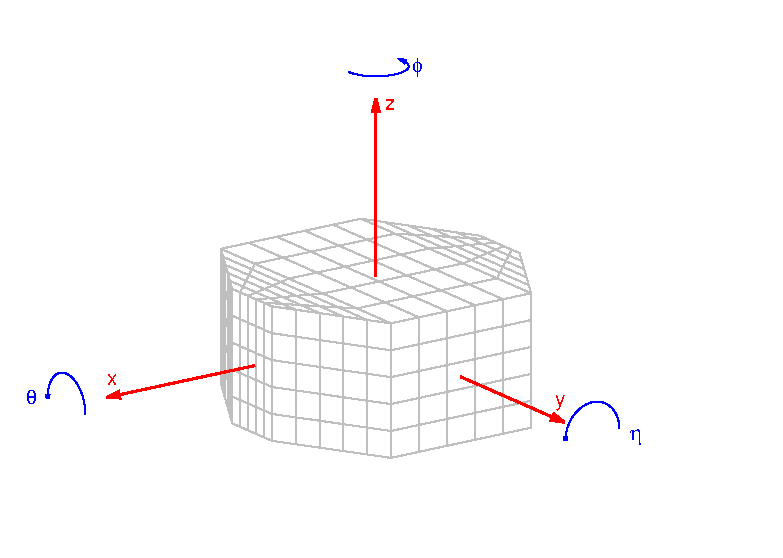
\includegraphics[width=0.5\textwidth]{figures/dof.eps}
%\caption{{\small Schematic showing the naming conventions for the six kinematic degrees of freedom used in this work. \red{not sure we really need a figure for this}}
%\label{fig:coordinates}
%\end{center}
%\end{figure}

%\FloatBarrier

\subsection{Impact Model and Sensitivity}
\label{sec:sensitivity}
The characteristic timescales of the impact process are short relative the sample cadence of the LPF data (typically $0.1\,\textrm{s}$). Consequently, we model the impact as a delta-function impulse in acceleration for each DoF.  These impulses occur at the same time for each DoF but have different amplitudes which encode information about the impact direction and location on the spacecraft. The modeling of the impact is performed in two steps. First, the acceleration in the S/C body frame is computed for both linear and angular DoFs:
\begin{eqnarray}
\vec{a}_{x,B}(t) = P\:M^{-1}\delta(t-\tau) \hat{e},\label{eq:axB} \\
\vec{a}_{\theta}(t)= P\:\mathbf{I}^{-1}\delta(t-\tau)\left(\vec{r}\times\hat{e}\right), \label{eq:aq}
\end{eqnarray}
where $\vec{a}_{x,B}$ is the acceleration of the spacecraft body frame in the linear DoFs, $\vec{a}_{\theta,B}$ is the acceleration of the spacecraft body frame in the angular DoFs, $P$ is the total transferred momentum, $\tau$ is the impact time, $\hat{e}$ is the unit-vector in the direction of the transferred momentum, $M$ is the mass of the S/C, $\mathbf{I}$ is the S/C moment of inertia about its center of mass, and $\vec{r}$ is the location of the impact relative to the center of mass. The angular accelerations at the TM locations are the same as described in (\ref{eq:aq}) but the linear accelerations pick up an additional term due to the offset of the test mass from the center of mass:
\begin{equation}
\vec{a}_{x,TM}(t) = \vec{a}_{x,B} + \left(\vec{r}_{TM}\times \vec{a}_{\theta}\right),\label{eq:axTM}
\end{equation}
where $\vec{a}_{x,TM}$ is the acceleration in the linear DoFs as measured in the test mass frame and $\vec{r}_{TM}$ is the location of the test mass relative to the S/C center of mass.

Sensitivity to impacts is limited by two noise sources: noise in the measurement system and disturbances on the S/C.  Measurement noise for both the capacitive and interferometric systems is characterized by a white spectrum in displacement whereas the chief noise source for the S/C disturbance, the micropropulsion system itself, exhibits an approximately white spectrum in force.  The relative levels of these two components differ for each DoF, but the basic functional form for the noise power spectral density is:
\begin{equation}
S_{g}=S_0+S_4f^4,
\label{eq:noise}
\end{equation}
where $S_0$ is the amplitude of the S/C disturbance term and $S_4$ is the amplitude of the measurement term. The most substantial difference between the noise level in the various DoFs is in the amplitude of the $S_4$ term, which is substantially lower for the DoFs sensed by the interferometric system: $x,\,\eta,$ and $\phi$.  In \cite{Thorpe:2015cxa} it was shown that SNR of a simple impulse in the presence of this noise shape can be analytically computed as $\rho =  P_i/P_c$, where $P_i$ is the amplitude of the momentum transfer in that DoF and $P_c$ is a characteristic threshold momentum given by:
\begin{equation}
P_c \equiv \frac{1}{\sqrt{2\pi}}\left(4 S_4 S_0^3\right)^{1/8}.\label{eq:SNRp}
\end{equation} 
The value of $P_c$ varies somewhat for each DoF due to the different combinations of sensing noise, micropropulsion noise, as well as differences in the spacecraft mass properties. The approximate range for linear DoFs is $0.05\,\mu\textrm{N-s}\leq P_c \leq 1\,\mu\textrm{N-s}$ and $0.3\,\mu\textrm{N-m-s}\leq P_c \leq 4\,\mu\textrm{N-m-s}$ for angular DoFs. This asymmetry in sensitivity along different DoFs means that impacts with lower overall momentum are often only detected in a fraction of DoF channels, meaning that the full set of parameters cannot be extracted. Similarly, impacts which happen to impart a large fraction of their momentum in a sensitive channel may be measured at lower thresholds than those coming from different directions.

%\FloatBarrier
\subsection{Detection and Parameter Estimation}\label{sec:MCMC}
The second step in our micrometeoroid pipeline involves the identification and characterization of candidate events in our data stream.  This is performed using the template-matching formalism that is commonly applied in gravitational wave data analysis. 
%Data model
Assuming the frequency domain data $\data$ contains an impact signal $\model$ plus noise $\n$, and $\n$ is zero-mean Gaussian distributed, the likelihood for observing  $\data$ is
\begin{equation}
p(\data|\params) = \prod_f \frac{1}{\det \Cij} e^{-\frac{1}{2}\sum_{ij} \residual_i \invCij \residual_j }
\label{eq:likelihood}
\end{equation}
where the $\residual = \data - \model(\params)$ is the residual, $\model(\params)$ is the modeled LISA Pathfinder response to an impact with parameters $\params$, and  $\Cij \equiv \langle \n_i \n_j\rangle$ is the one-sided noise correlation matrix. The indices $i$ and $j$ sum over different data channels, i.e. the 6 degrees of freedom $i:=(x,y,z,\theta,\eta,\phi)$.

%Noise model
We make the simplifying assumption that the noise correlation matrix $\Cij$ is diagonal, i.e. that the noise in each channel is independent. While this is likely a reasonable assumption for the sensing noise component, the platform noise may be somewhat correlated due to common contributions from the micropropulsion system. 
We further assume that the noise in each channel is stationary, implying that there are no  correlations between different frequencies, and the noise is completely characterized by its variance.
\begin{equation}
\langle \n^2(f)\rangle \equiv \frac{T}{2}S_n(f)
\end{equation}
where $T$ is the duration of the data segment and $S_n(f)$ is the one-sided noise power spectral density.
For flexibility to fit realistic instrument noise, we use a phenomenological model for $S_n(f)$ rather than the theoretical form in Eq.~\ref{eq:noise}.
The model is adopted from the BayesLine algorithm~\citep{Littenberg_15} used for spectral estimation in analysis of transient sources detected by the ground-based gravitational wave detector network.
BayesLine is a trans-dimensional (or reversible jump) Markov Chain Monte Carlo (MCMC) algorithm~\citep{Green_95}.
The spectral noise model is built from two-components:  the broad band spectral shape is fit with a cubic spline interpolation, where the number and location of spline control points are free parameters; and a linear combination of  Lorentzians to fit narrow band spectral lines that were present when the cold gas micropropulsion system was active \citep{ST7_Results}.
The model is flexible, and proved to be well suited for fitting the LISA Pathfinder noise.

%Signal model
The signal model was implemented as described in Sec.~\ref{sec:sensitivity}, again using a trans dimensional MCMC.
The MCMC samples between hypothesis that the data contain only noise (i.e. that there is no impact signal in the model) or that the data contain noise and a single impact.
The ratio of MCMC iterations spent in the two hypothesis is the Bayes factor, or marginalized likelihood ratio, between the signal and the noise model.
We use the Bayes factor $B_{\rm signal,noise}$ as the detection statistic, with a threshold of $B_{\rm signal,noise} > 3{:}1$ for claiming a positive detection.
The Markov chain's samples from iterations which included the signal hypothesis are used to characterize the posterior distribution function of the impact parameters, conditional on a signal actually being present in the data.
Marginalized posterior distributions for the incident direction of the impact, and the momentum imparted to the spacecraft, are used to make further inferences about the micrometeorite population.
The priors for the signal parameters are uniform distributions in time, imparted momentum, impact location, and incident direction of the impact.  

%MCMC validation
Both the noise model and signal model MCMC samplers use parallel tempering to improve the convergence time of the chains.
The MCMC code went through a standard suite of tests to confirm that the results are accurate and robust.
The spectral estimation code is validated by testing that the whitened data $\data(f)/\sqrt{S_n(f)}$ are consistent with being drawn from a zero mean, unit variance, Gaussian.
We check detailed balance of the sampler by using a constant likelihood function and testing that the recovered distributions are consistent with the priors.
Finally, the samplers are tested for accuracy by analyzing simulated and real data with artificial signals added, verifying that the true signal parameters are included in the posterior distributions.
 
%Caveats
The noise and impact models used in this analysis are not perfect and further advancements may improve the detection efficiency and/or reduce systematic errors in parameter recovery.
A particular weakness is our assumption that the noise in each channel is independent. 
The sensing degrees of freedom are not the same as the kinematic degrees of freedom, so noise correlations are not necessarily negligible. 
We also found that, for large momentum impacts, a noticeable residual was left in the data, indicating that our signal model was not a perfect match to the data. 
This modeling mismatch results in an uncharacterized systematic error, though the macroscopic conclusions drawn from the posterior--which face of the spacecraft was impacted, from what (general) region of the sky did the impactor originate, and the overall distribution of imparted momenta of the impactors--are not expected to be biased to the point of misleading the general conclusions.
Improvements to the model, especially developing a physically motivated forward model of the instrument noise, are areas for future study.


%\FloatBarrier
\begin{figure*}[t]
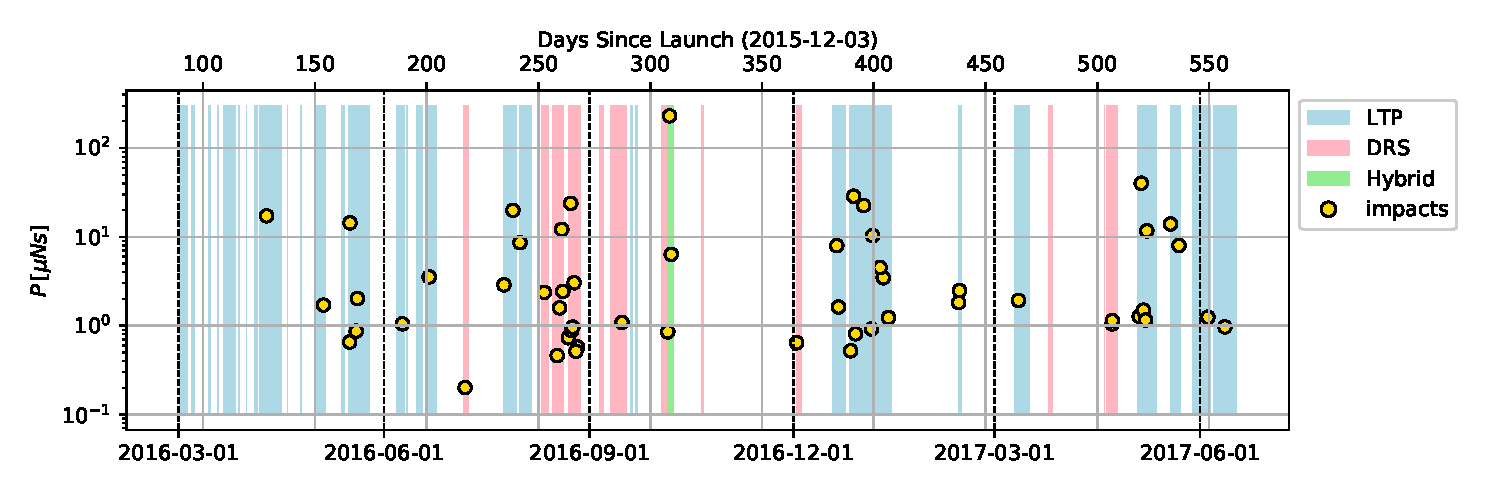
\includegraphics[width=\textwidth]{figures/timeline.eps} 
\caption{Timeline of impact events during LPF. The yellow dots show the impact times with the total transferred momentum defining the vertical axis. The vertical bars denote the times included in the search with blue representing the nominal LTP configuration, pink the DRS configuration, and green the hybrid configuration. See text for details. \label{fig:timeline}}
\end{figure*}

\subsection{Post processing and vetos}\label{sec:vetos}
For each segment of data, the MCMC tool described in Section \ref{sec:MCMC} was run for in an initial search comprised of $7\times10^4$ steps on the TM1 data. After discarding the first $3\times10^4$ steps of the chain as ``burn in'' samples, the detection fraction was computed as the ratio of chain steps where an impact model was included to the total number of steps.  For systems with a detection fraction above 0.5, the MCMC tool was re-run in a characterization step of $7\times10^5$ steps on both TM1 and TM2. A burn-in period of $3.5\times10^5$ steps was discarded from both chains and the detection fraction was again computed as well as the variance in the impact time parameter $\tau$.  For systems with an above-threshold detection fraction and impact time variance of less than 0.3\,s in both TMs were passed on to the next step in the vetting process, manual inspection.  For the manual inspection process, an expanded set of telemetry from the spacecraft around the candidate impact time was downloaded and examined.  Examples of signals inspected include all force and torque signals, all position and attitude signals, selected voltage levels, and internal telemetry of the micropropulsion system. This process yielded two types of false triggers: thruster current spikes and data gaps. Candidates for which the signals appeared consistent with expectations were added to the catalog.

For vetted impact candidates, an additional post-processing step was conducted to extract parameters of interest.  In order to compare with the micrometeoroid population models in Section \ref{sec:models}, it was necessary to transform the impact direction from S/C coordinates to the Sun-Tracking Ecliptic Frame used by the micrometeoroid population models.  This transformation was done in two steps, first from the S/C frame to an Earth-Centered Inertial (ECI) frame using the S/C quaternion telemetry provided by the star tracker, and then from ECI to the Sun-Tracking Ecliptic Frame using the S/C ephemeris. Median sky location and a 90\% confidence sky area for both frames was computed using HEALPIX\citep{HEALPIX}. 

\begin{figure}[t]
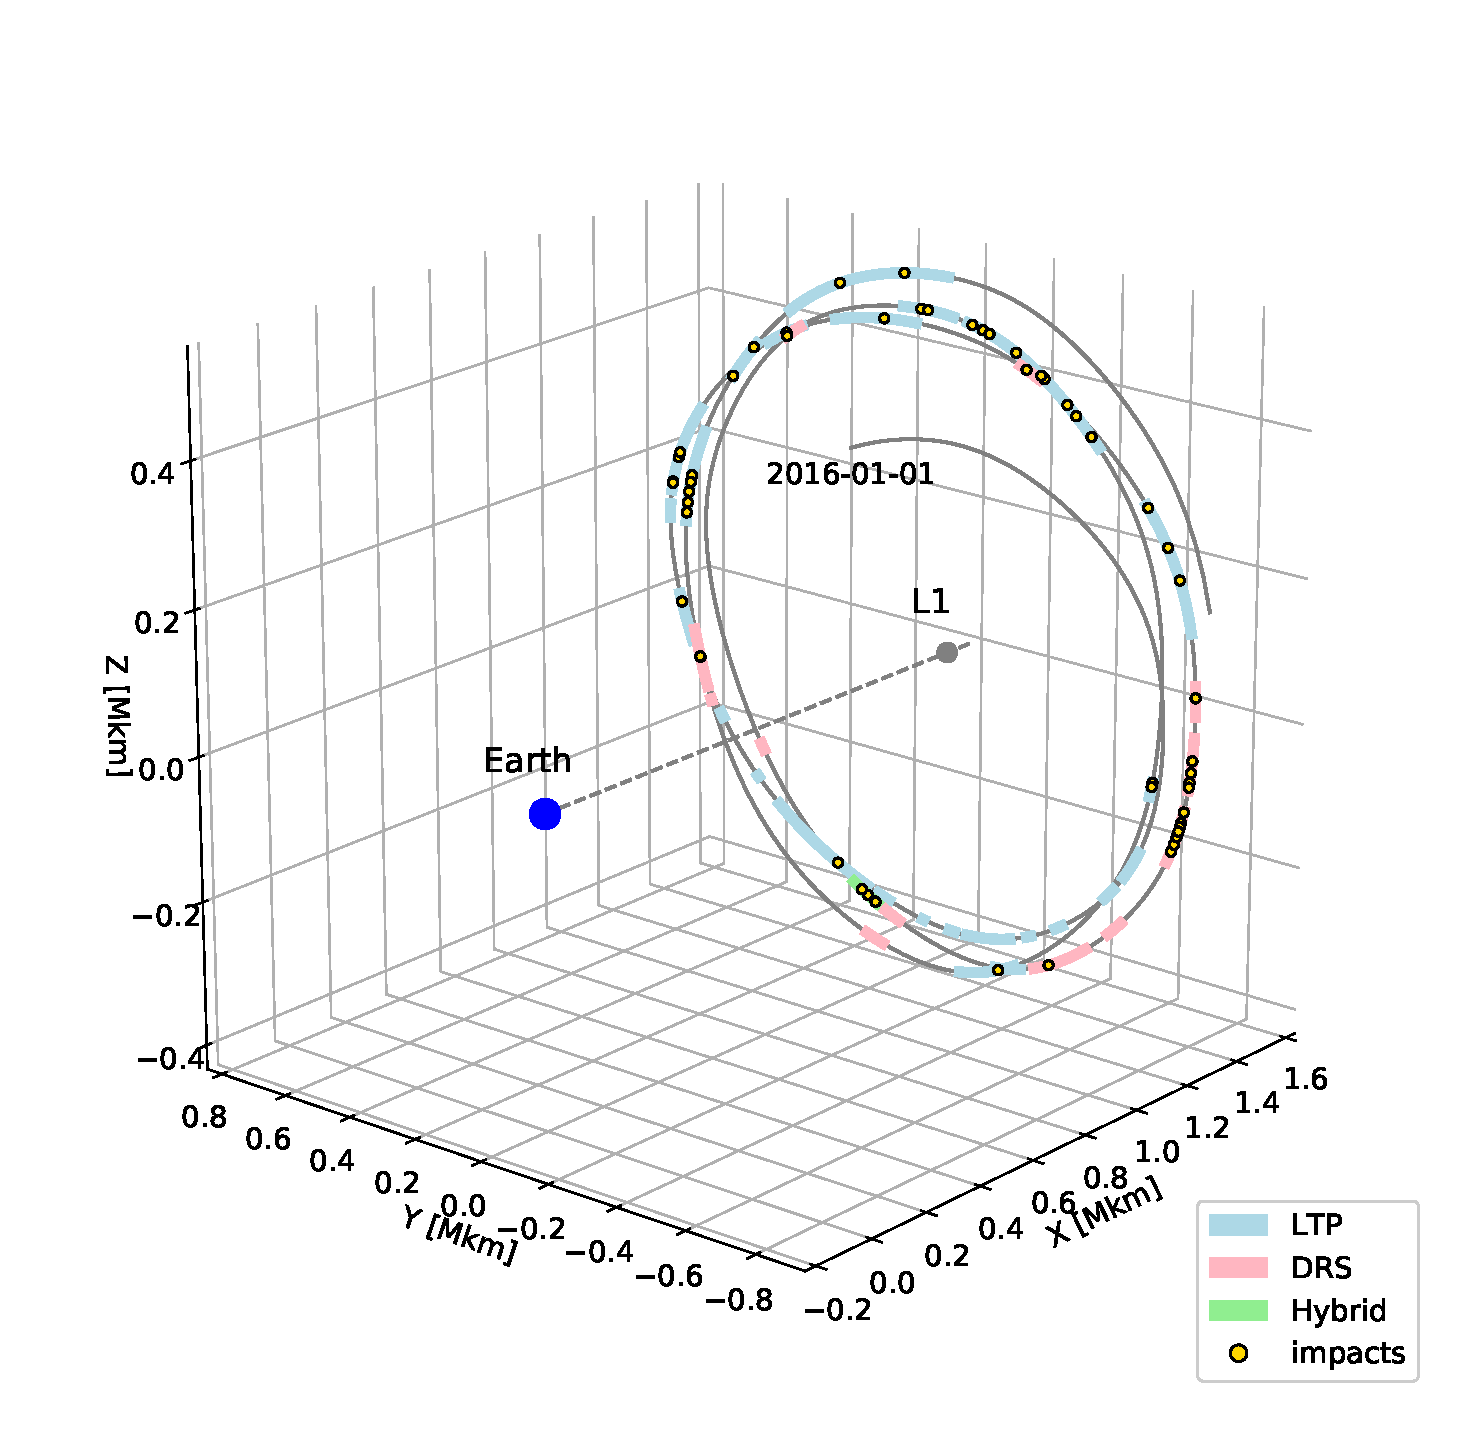
\includegraphics[width=\columnwidth]{figures/ephemeris.eps} 
\caption{Micrometeoroid impacts visualized along LPF's trajectory as plotted in an Earth-Centered, Sun-synchronous frame.  The solid gray line shows LPF's clockwise trajectory from 2016-01-01 through 2017-07-31 with the times searched for impacts in the LTP, DRS, and hybrid configurations in blue, pink, and green respectively. Impacts are indicated by yellow circles. \label{fig:ephemeris}}
\end{figure}

\section{Results} \label{sec:results}
In this paper we restrict our analysis to segments of data where no signals were deliberately injected into the LPF system. We identified a total of \nhours hours of data in three distinct configurations: the nominal LPF configuration in which the European-provided DFACS control system and cold gas micropropulsion system were operating (3484 hours), the DRS configuration in which the NASA-provided DCS control system and colloidal micropropulsion system were operating (796 hours), and a hybrid configuration in which the DFACS was controlling the S/C using the colloidals (61 hours). Figure \ref{fig:timeline} shows a timeline of these segments along with the detected impacts plotted with their total transferred momentum along the vertical axis. The total number of detected impacts is 54: 36 in the nominal configuration, 15 in the DRS configuration, and 3 in the hybrid configuration. This corresponds to a rough event rate of 120 yr$^{-1}$, which is broadly consistent with the estimate made in \cite{Thorpe:2015cxa} as well as the models in Section \ref{sec:models}.  Figure \ref{fig:ephemeris} shows the timeline from Figure \ref{fig:timeline} projected onto the LPF ephemeris from 2016-01-01 through 2017-03-31 in an Earth-centered, Sun-synchronous frame.
 
In the following sections we present some example events in detail and summarize some properties of the observed population.  A full catalog of the impacts and their estimated parameters can be found in Appendix A.

\subsection{Sample candidate events \label{sec:samples}}
As mentioned in Section \ref{sec:sensitivity}, LPF's sensitivity depends on the parameters of the impact including both the total momentum transferred as well as the fraction of that momentum that is  projected into each DoF.  As a result, the quality of our parameter estimation varies greatly from impact to impact.  Figures \ref{fig:goodExampleCorner} and \ref{fig:goodExampleLocation} show results for an impact occurring at GPS time $t_{gps}=1154024345.4$, corresponding to 2016-07-31 18:18:48.400 UTC. 

With a moderately high transferred momentum of $8.5\,\mu\textrm{N-s}$ and a S/C longitude that aligns well with the sensitive x-axis, the total SNR in the two TMs are $\rho_1\approx16$ and $\rho_2\approx22$ . Figure \ref{fig:goodExampleCorner} shows an overlaid corner plot representing the posterior probabilities for the impact parameters as measured by TM1 (in red, lower-left) and TM2 (in blue, upper-right).  The panels are arranged in a grid with rows and columns corresponding to the following parameters: total transferred momentum ($P_{tot}$, in $\mu$N-s), S/C latitude defined relative to the S/C x-y plane ($lat$, in deg.), S/C longitude defined relative to the +x axis ($lon$, in deg.), and x,y,z, locations of the impact with respect to the S/C center of mass ($r_x,\,r_y,\,r_z$ in $m$).  The panels along the diagonal show the posterior probability density for each parameter as measured by TM1 (red) and TM2 (blue).  The panels on the off-diagonals show the correlation between pairs of parameters in the TM1 data (lower off-diagonals) and TM2 data (upper off-diagonals). The measured parameters between these two impacts are broadly consistent, although TM1 generally prefers a solution with slightly increased $P_{tot}$, larger $lat$, and positive shifts in both $r_x$ and $r_z$. 

Figures \ref{fig:typExampleCorner} and \ref{fig:typExampleLocation} show a similar set of plots as Figures \ref{fig:goodExampleCorner} and \ref{fig:goodExampleLocation} but for an impact occurring at $t_{gps} = 1149475987.7$ (2016-06-09 02:52:50.700 UTC) which had a lower total momentum ($P_{tot}\approx1.0\,\mu\textrm{N-s}$), and lower SNR ($\rho_1\approx1.5$, $\rho_2\approx1.4$). As a result, the constraints on parameters other than the total momentum are rather weak.  The impact location is favored towards the -x and +z faces and the preferred direction to the impactor is in the direction from the Sun (latitudes around 0 deg) and above the ecliptic. These parameters are also suggestive of a JFC-type impactor, although the less-common Asteroidal type would be consistent with the observed geometry.

%\FloatBarrier

\begin{figure*}[ht!]
\gridline{
\fig{figures/goodDualCorner.eps}{\textwidth}{}}
\vspace*{-20mm}
\caption{Comparison of recovered posterior distributions for impact parameters using TM1 and TM2 data for the impact candidate occurring at $t_{gps}=1154024345.4$, which is representative of a well-characterized event in our catalog. The array of plots is organized by parameter with a parameter order from left-to-right and top-to-bottom of total momentum transfer, latitude and longitude of impact direction in  spacecraft frame, and x,y,z location of impact with respect to S/C center of mass. Diagonal panels show single-parameter probability density functions with TM1 data in red and TM2 data in blue. Lower corner panels (red shades) show 2-parameter histograms for TM1 while upper corner panels (blue shades) show 2-parameter histograms for TM2. \label{fig:goodExampleCorner}}
\end{figure*}

\begin{figure*}[ht!]
\gridline{
\fig{figures/badDualCorner.eps}{\textwidth}{}}
\vspace*{-20mm}
\caption{Comparison of recovered posterior distributions for impact parameters using TM1 and TM2 data for the impact candidate occurring at $t_{gps}=1149475987.7$, which is representative of a typically characterized event in our catalog. The plot arrangement is the same as Figure \ref{fig:goodExampleCorner}.\label{fig:typExampleCorner}}
\end{figure*}

\begin{figure*}[h!]
\gridline{
\fig{figures/goodSky.eps}{0.5\textwidth}{(a) Impact origin in Sun-tracking Ecliptic Frame}
\rotatefig{90}{figures/goodFlat.eps}{0.37\textwidth}{(b) Impact location on S/C}}
\caption{Reconstructed impact direction and location using TM1 data for impact candidate occurring at $t_{gps}=1154024345.4$. Color contours denote fraction of post-burn-in MCMC samples in each bin.\label{fig:goodExampleLocation}}
\end{figure*}

\begin{figure*}[h!]
\gridline{
\fig{figures/badSky.eps}{\columnwidth}{(a) Impact origin in Sun-tracking Ecliptic Frame }
\rotatefig{90}{figures/badFlat.eps}{0.37\textwidth}{(b) Impact location on S/C}}
\caption{Reconstructed impact direction and location using TM1 data for impact candidate occurring at $t_{gps}=1149475987.7$. Color contours denote fraction of post-burn-in MCMC samples in each bin.\label{fig:typExampleLocation}}
\end{figure*}


\subsection{Ensemble results}
In this section, we describe some of the properties of our observed ensemble of events and make some comparisons to the model populations described in Section \ref{sec:models}. 

Micrometeoroid impact times are expected to be governed by a Poisson process characterized by a single rate parameter.  Figure \ref{fig:CDF_rate} shows the cumulative probability density of the observed time between events, which was computed from mission elapsed time by excising the times not included in our search. As is expected for a Poisson process, this distribution follows an exponential function, with a time between events of $2.94\pm0.05\,$days or a rate of $(124\pm2)\,\textrm{yr}^{-1}$.  This is consistent with the predictions in Section \ref{sec:models}.

From the observed impacts, we perform a hierarchical analysis to infer properties of the imparted momentum distribution and, assuming totally inelastic collisions, the momentum distribution of the micrometeorite population.
We select only impacts with measured momenta $P>P_{\rm min}=1\ \mu N s$ as a threshold above which we assume 100\% detection efficiency and therefore neglect selection effects.
The marginalized posteriors of the momenta from the MCMC analysis described in section \ref{sec:MCMC} are approximated as Gaussian distributions with mean and variance computed from the Markov chains.
The approximate posteriors become the data $d$ in a hierarchical analysis which compares three models for the probability density function of momenta: 
A single power law 
\begin{equation}
p(P;\alpha) = A( P / P_{\rm min} )^{-\alpha}
\end{equation}
a broken power law with fixed ``knee'' momentum $P^*$
\begin{equation}
p(P;\alpha,\beta) =
\begin{cases}
 A( P / P_{\rm min} )^{-\alpha} & \text{if $P \leq P^*$}\\
B( P / P_{\rm min} )^{-\beta} & \text{else }
\end{cases}
\end{equation}
and a three parameter model $p(P;\alpha,\beta,P^*)$ with adjustable knee location, where $A$ and $B$ normalize the distributions.
A MCMC code is used to characterize each model, and from the maximum likelihood we compute the Bayesian Information Criterion (BIC)~\citep{schwarz1978}. The model which minimizes the BIC is preferred.




\begin{figure}[h!]
\gridline{\fig{figures/rateplot.eps}{0.5\textwidth}{}}
\vspace*{-8mm}
\caption{Cumulative distribution of observed time interval between events, taking into account gaps in the observations. The red curve is an exponential fit with a characteristic interval between events of $2.94\pm0.05\,$days. \label{fig:CDF_rate}}
\end{figure}


For these data, the one-parameter model is selected, with BIC scores of 48, 53, and 56  for $p(P;\alpha)$, $p(P;\alpha,\beta)$, and $p(P;\alpha,\beta,P^*)$, respectively. 
As a sanity check, we also confirmed that the marginalized posteriors $p(\alpha | d)$ and $p(\beta | d)$ were largely overlapping (or, the posterior $p(\alpha-\beta|d)$ peaks near zero) as would be expected in the case where the one-parameter model adequately described the data.
The spectral index is measured to be
%$\alpha = 1.86722^{2.07707}_{1.67904}$ more digits if you want them
$\alpha = 1.87^{2.08}_{1.68}$ 
quoted as the median with upper and lower 90\% credible intervals from the posterior distribution function as super- and sub-scripts.

Figure \ref{fig:PDF_P} shows the inferred posterior distribution as a histogram of the chain samples (light blue-green) and a Kernel Density Estimate (dark blue-green) from the single-power-law model on $\alpha$. The vertical dashed lines (orange) mark the 90\% credible intervals.  The four vertical lines (purple) are the best-fit power-law indices for the different micrometeorite progenitors as shown in Table~\ref{tab:popCDFfits}. The OCC model (dash-double-dotted line) is disfavored by these observations. Figure \ref{fig:CDF_P} shows a comparison of the cumulative distribution of impact momenta from the Kernel Density Estimate (1-,2-, and 3-$\sigma$ intervals as solid, dashed, and dot-dashed lines respectively) with the measured distribution of the individual impacts, shown in green with 90\% error bars from the individual MCMC posteriors. 

\begin{figure}[h!]
%\gridline{\fig{figures/momentumCDF.png}{0.5\textwidth}{}}
\gridline{\fig{figures/power_law_posterior_compare.pdf}{0.5\textwidth}{}}
\vspace*{-8mm}
\caption{Inferred posterior distribution for momentum of underlying micrometeoroid population as a histogram of the chain samples (light blue-green) and a Kernel Density Estimate (dark blue-green) from a single-power-law model. The vertical dashed lines (orange) mark the 90\% credible intervals.  The four vertical lines (purple) are the best-fit power-law indices for the different micrometeorite progenitors as shown in Table~\ref{tab:popCDFfits}. The OCC model (dash-double-dotted line) is disfavored by these observation. See text for details. \label{fig:PDF_P}}
\end{figure}

\begin{figure}[h!]
\gridline{\fig{figures/pvalue_quantiles_paper.pdf}{0.5\textwidth}{}}
\vspace*{-8mm}
\caption{Cumulative distribution of impact momenta from the 54 measured events (green points with 90\% credible error bars from individual MCMC posteriors) as well as 1-, 2-, and 3-$\sigma$ ranges for the underlying distribution generated using the Kernel Density Estimate. These can be directly compared with the model distributions in Figure \ref{fig:popCDF}. See text for details. \label{fig:CDF_P}}
\end{figure}



A second way to distinguish against potential populations is to compare the distribution of events on the sky.  As mentioned in Section \ref{sec:sensitivity}, LPF's ability to localize events on the sky depends on detecting and measuring momentum transfer in multiple degrees of freedom. This is more likely to occur as the overall transferred momenta increases. Indeed, we find a correlation between total momentum and area of the 68\% confidence sky position of $\delta A\approx1.5\times10^4\,\textrm{deg}^2\,\left(P/1\,\mu\textrm{N}\right)^{-0.74}$. The main panel of figure \ref{fig:mapCompare} shows the measured sky position with 68\% error bars for the subset of 14 events for which the area of the 68\% confidence region on the sky is less than 4125$\,\textrm{deg}^2$ or 10\% of the sky. The top panel shows in gray a histogram of the events in 15$^\circ$ bins of latitude as well as the modeled flux distribution for impacts with momentum $\geq 1\,\mu$Ns for the JFC (blue), HTC (orange), OCC (green), and AST (red) populations. Right panel is similar to the top panel but for latitude in 30$^\circ$ bins.  While the limited number of well-localized events makes it difficult to quantitatively compare the data to the models, the distribution of events is suggestive of the JFC population, particularly in latitude. 

\begin{figure}[h!]
\gridline{\fig{figures/mapCompare.eps}{0.5\textwidth}{}}
\vspace*{-8mm}
\caption{Comparison of sky distribution of localized events with population models. Main panel shows sky locations for the subset of (14) events which were localized to an area within 10\% of the sky including error bars spanning a 68\% confidence level. Top panel shows in gray a histogram of the events in 15$^\circ$ bins of latitude as well as the modeled flux distribution for impacts with momentum $\geq 1\,\mu$Ns for the JFC (blue), HTC (orange), OCC (green), and AST (red) populations. Right panel is similar to the top panel but for latitude in 30$^\circ$ bins. See text for details. \label{fig:mapCompare}}
\end{figure}




%\FloatBarrier
\section{Population Model Inference} \label{sec:model_inference}
To improve upon the qualitative nature of the model comparison in Figure \ref{fig:mapCompare} and make a more qualitative statement about the agreement between the models in section \ref{sec:models} and LPF's observations, a hierachircal Bayesian model was developed that utilized the momentum and sky distribution of each population model to assess the likelihood that any particular step in the impact search chain was associated with an impact from a specific population.  This machinery was then applied to the \emph{entire} set of cleaned LPF data, including segments for which no impact was positively identified (but excluding the few vetoed events). This is an important advantage as non-detection of an event when a model predicts likely detections can be as important to model selection as detection of such events. The hierachircal model, which is described in detail in Appendix B, assumes that the underlying population of micrometeoroids is a mixture of a set of sub-populations and measures the posterior distributions of the relative contributions of these populations.  

In Figure~\ref{fig:bayes} we show the resulting Bayes factors for models composed of mixtures of the JFC, HTC, and OCC population models as well as a Uniform sky model which is used as a control.  The parameters of the hierarchical models are the fraction of net micrometeoroid flux assumed from each sub-population, with the overall rate fixed to the observed rate. In the Figure~\ref{fig:bayes}(a), we consider models composed of a mixture of the JFC, HTC, and OCC sub-populations.  The result shows that models favoring predominantly JFC micrometeoroids are strongly favored while models with a large fraction of OCC micrometeoroids are especially disfavored.  The roughly 2:1 ratio of JFCs to HTCs predicted by the models outlined in section \ref{sec:models} lies in the region of maximum likelihood. The dominance of the combined JFC+HTC combinations over the OCC population is also consistent with these models so long as the threshold for observed impacts is greater than a few $\mu$N-s.  Figure~\ref{fig:bayes}(b) shows results from a hierarchical model consisting of JFC, HTC, and Uniform-sky subpopulations. Models dominated by JFC micrometeoroids are again strongly favored.  
%
\begin{figure*}[ht!]
\gridline{\fig{figures/grid_OCC_JFC_HTC_20190219.pdf}{\columnwidth}{(a) Sub-population ratio distribution with JFC, HTC and OCC components}
\fig{figures/grid_JFC_HTC_Uniform_20190219.pdf}{\columnwidth}{(b) Sub-population ratio distribution with JFC, HTC and Uniform components}}
\caption{These figures show log Bayes factors for model comparisons with varying fractional contributions from our sub-population models. Differences of more than a few begin to be significant with a difference of 20 indicating very strong evidence.
  Panel a) shows most-probable relative rates of $\sim$80-90\% JFC with $\sim$10-20\% HTC micrometeoroids and no significant contribution from OCC.  Panel b) considers an alternative less-informed model leaving out the OCC sub-population, but allowing the possibility of an additional sub-population which is uniformly distributed across the sky. Models dominated by the JFC share of the micrometeoroids remain strongly favored. \label{fig:bayes}}
\end{figure*}

%\FloatBarrier
\section{Conclusions} \label{sec:conclusions}
We have presented a comprehensive analysis of micrometeoroid impacts detected by the LISA Pathfinder spacecraft using a novel technique - direct measurement of the momentum transfer from an individual microscopic impactor to a spacecraft. This data set, although limited to a handful of events, provides an interesting new source of data for the zodiacal dust complex, an important component of our Solar System.  The population observed by LPF is broadly consistent with standard models of the micrometeoroid population, suggesting that such models are appropriate for use in estimating hazards for spacecraft operating in the inner solar system.  A statistical comparison of our data set with model predictions favors models dominated by Jupiter-family Comets  with a potential smaller contribution from Halley-type Comets. This is broadly consistent with standard models of the zodiacal dust complex although our statistical evidence limited.  This same technique may be utilized by future precision-measurement missions, most notably the Laser Interferometer Space Antenna (LISA) itself, which based on this analysis will observe many more micrometeoroid impacts due to its combination of more spacecraft, larger spacecraft, and longer observing time - providing an additional science benefit beyond the compelling science case for observing the universe in the milliHertz gravitational wave band.

%% If you wish to include an acknowledgments section in your paper,
%% separate it off from the body of the text using the \acknowledgments
%% command.
\acknowledgments

This analysis was conducted under a 2017 NASA Science Innovation Fund awarded to Thorpe, Littenberg, Janches, and Baker. Slutsky acknowledges support of the NASA Astrophysics Division. Pagane and Hourihane acknowledge the support of the NASA Undergraduate Summer Internship program and Hourihane acknowledges the support of the National Science Foundation's Research Experience for Undergraduates program.
\\

The data was produced by the LISA Pathfinder mission, which was part of the
space-science programme of the European Space Agency and also hosted the NASA Disturbance Reduction System payload, developed under the NASA New Millennium Program. 

The French contribution to LISA Pathfinder has been supported by the CNES (Accord Specific de projet
CNES 1316634/CNRS 103747), the CNRS, the Observatoire de Paris and the University
Paris-Diderot. E.~Plagnol and H.~Inchausp\'{e} would also like to acknowledge the
financial support of the UnivEarthS Labex program at Sorbonne Paris Cit\'{e}
(ANR-10-LABX-0023 and ANR-11-IDEX-0005-02).

The Albert-Einstein-Institut acknowledges the support of the German Space Agency,
DLR, in the development and operations of LISA Pathfinder. The work is supported by the Federal Ministry for Economic Affairs and Energy
based on a resolution of the German Bundestag (FKZ 50OQ0501 and FKZ 50OQ1601). 

The Italian contribution to LISA Pathfinder has been supported  by Agenzia Spaziale Italiana and Istituto
Nazionale di Fisica Nucleare.

The Spanish contribution to LISA Pathfinder has been supported by contracts AYA2010-15709 (MICINN),
ESP2013-47637-P, and ESP2015-67234-P (MINECO). M.~Nofrarias acknowledges support from
Fundacion General CSIC (Programa ComFuturo). F.~Rivas acknowledges an FPI contract
(MINECO).

The Swiss contribution to LISA Pathfinder was made possible by the support of the Swiss Space Office (SSO)
via the PRODEX Programme of ESA. L.~Ferraioli is supported by the Swiss National
Science Foundation.

The UK LISA Pathfinder groups wish to acknowledge support from the United Kingdom Space Agency
(UKSA), the University of Glasgow, the University of Birmingham, Imperial College,
and the Scottish Universities Physics Alliance (SUPA).

%% To help institutions obtain information on the effectiveness of their 
%% telescopes the AAS Journals has created a group of keywords for telescope 
%% facilities.
%
%% Following the acknowledgments section, use the following syntax and the
%% \facility{} or \facilities{} macros to list the keywords of facilities used 
%% in the research for the paper.  Each keyword is check against the master 
%% list during copy editing.  Individual instruments can be provided in 
%% parentheses, after the keyword, but they are not verified.

\vspace{5mm}
\facilities{LPF (\url{http://sci.esa.int/lisa-pathfinder/})}

%% Similar to \facility{}, there is the optional \software command to allow 
%% authors a place to specify which programs were used during the creation of 
%% the manusscript. Authors should list each code and include either a
%% citation or url to the code inside ()s when available.

\software{LTPDA (\url{https://www.elisascience.org/ltpda/}), \:
MATPLOTLIB (\url{https://matplotlib.org/}),\:
HEALPY (\url{https://github.com/healpy/healpy}),\:
ligo.skymap (\url{https://lscsoft.docs.ligo.org/ligo.skymap})}

%% Appendix material should be preceded with a single \appendix command.
%% There should be a \section command for each appendix. Mark appendix
%% subsections with the same markup you use in the main body of the paper.

%% Each Appendix (indicated with \section) will be lettered A, B, C, etc.
%% The equation counter will reset when it encounters the \appendix
%% command and will number appendix equations (A1), (A2), etc. The
%% Figure and Table counter will not reset


 \appendix
 \section{List of Impact Events in LPF}
The catalog of LPF impact events is reported in the table below. For each impact, the date of impact, GPS timestamp, and median inferred momentum transfer with 95\% confidence intervals are listed. For impacts with an inferred 95\% confidence sky location of less than 4100 $deg^2$ (10\% of the sky), the 95\% error area as well as the impact direction in both spacecraft and Sun Synchronous Ecliptic Coordinates is reported. For impacts with a greater than 75\% probability of impacting on a particular face of the spacecraft, the spacecraft face is identified. The location of LPF in its orbit at the time of the impact is provided in EME2000 (J2000) coordinates. 
			\begingroup
			\renewcommand\arraystretch{2}
			\begin{longtable*}{|c|c|c|c|c|c|c|c|c|c|c|c|}

				\hline 
				& 
				& 
				& 
				&
				&
				\multicolumn{4}{|c|}{Sky Location} &
				\multicolumn{3}{|c|}{LPF Position (EME2000)} \\
				\multicolumn{1}{|c}{Date} & 
				\multicolumn{1}{|c|}{GPS [s]}  & 
				\multicolumn{1}{|c|}{$P_{med}$} & 
				\multicolumn{1}{|c|}{Face} &
				\multicolumn{1}{|c|}{Localization} &
				\multicolumn{1}{|c|}{$Lat_{SC}$} &
				\multicolumn{1}{|c|}{$Lon_{SC} $} &
				\multicolumn{1}{|c|}{$Lat_{SSE}$} &
				\multicolumn{1}{|c|}{$Lon_{SSE}$} &
				\multicolumn{1}{|c|}{$X$} &
				\multicolumn{1}{|c|}{$Y$} &
				\multicolumn{1}{|c|}{$Z$} \\
				& 
				[s] & 
				$[\mu N s]$& 
				&
				$[deg^2]$&
				\multicolumn{1}{|c|}{$[deg]$} &
				\multicolumn{1}{|c|}{$ [deg]$} &
				\multicolumn{1}{|c|}{$[deg]$} &
				\multicolumn{1}{|c|}{$[deg]$} &
				\multicolumn{1}{|c|}{$[Mkm]$} &
				\multicolumn{1}{|c|}{$[Mkm]$} &
				\multicolumn{1}{|c|}{$[Mkm]$} \\
				\hline
			\endfirsthead
			        
				\multicolumn{12}{r}{continued from previous page} \\
				\hline 
				& 
				& 
				& 
				&
				&
				\multicolumn{4}{|c|}{Sky Location} &
				\multicolumn{3}{|c|}{LPF Position (EME2000)} \\
				\multicolumn{1}{|c}{Date} & 
				\multicolumn{1}{|c|}{GPS [s]}  & 
				\multicolumn{1}{|c|}{$P_{med}$} & 
				\multicolumn{1}{|c|}{Face} &
				\multicolumn{1}{|c|}{Localization} &
				\multicolumn{1}{|c|}{$Lat_{SC}$} &
				\multicolumn{1}{|c|}{$Lon_{SC} $} &
				\multicolumn{1}{|c|}{$Lat_{SSE}$} &
				\multicolumn{1}{|c|}{$Lon_{SSE}$} &
				\multicolumn{1}{|c|}{$X$} &
				\multicolumn{1}{|c|}{$Y$} &
				\multicolumn{1}{|c|}{$Z$} \\
				& 
				[s] & 
				$[\mu N s]$& 
				&
				$[deg^2]$&
				\multicolumn{1}{|c|}{$[deg]$} &
				\multicolumn{1}{|c|}{$ [deg]$} &
				\multicolumn{1}{|c|}{$[deg]$} &
				\multicolumn{1}{|c|}{$[deg]$} &
				\multicolumn{1}{|c|}{$[Mkm]$} &
				\multicolumn{1}{|c|}{$[Mkm]$} &
				\multicolumn{1}{|c|}{$[Mkm]$} \\	
				\hline		
				\endhead
			
			\hline 
			\multicolumn{12}{|r|}{{Continued on next page}} \\ 
			\hline
			\endfoot

			\hline
			\endlastfoot
	2016-04-09 & 1144229908 & $17.2^{+0.4}_{-0.3}$ & +y+y & 1729 & -7 & -7 & -57 & -39 & 1.09 & 0.55 & -0.05 \\
	2016-05-04 & 1146429822 & $ 1.7^{+3.1}_{-0.6}$ & - & - & - & - & - & - & 0.45 & 1.24 & 0.56 \\
	2016-05-16 & 1147442122 & $ 0.7^{+0.5}_{-0.5}$ & - & - & - & - & - & - & 0.14 & 1.34 & 0.77 \\
	2016-05-16 & 1147453726 & $14.4^{+0.8}_{-0.4}$ & +x+x & 3438 & -2 & 162 & 45 & -56 & 0.14 & 1.34 & 0.77 \\
	2016-05-19 & 1147693044 & $ 0.9^{+0.9}_{-0.3}$ & - & - & - & - & - & - & 0.08 & 1.35 & 0.81 \\
	2016-05-19 & 1147741578 & $ 2.0^{+0.8}_{-0.3}$ & - & - & - & - & - & - & 0.06 & 1.35 & 0.82 \\
	2016-06-08 & 1149475988 & $ 1.0^{+1.1}_{-0.3}$ & - & - & - & - & - & - & -0.26 & 1.36 & 1.00 \\
	2016-06-20 & 1150511110 & $ 3.5^{+1.7}_{-1.2}$ & - & - & - & - & - & - & -0.35 & 1.33 & 1.03 \\
	2016-07-07 & 1151901050 & $ 0.2^{+0.5}_{-0.1}$ & - & - & - & - & - & - & -0.42 & 1.35 & 1.00 \\
	2016-07-24 & 1153404058 & $ 2.9^{+1.3}_{-0.3}$ & - & - & - & - & - & - & -0.48 & 1.37 & 0.87 \\
	2016-07-28 & 1153750663 & $19.9^{+1.7}_{-1.3}$ & +z+z & 2585 & 18 & 158 & -31 & -172 & -0.51 & 1.38 & 0.83 \\
	2016-07-31 & 1154024345 & $ 8.6^{+1.8}_{-1.6}$ & +x+y & 3857 & -7 & 128 & -7 & 156 & -0.54 & 1.38 & 0.79 \\
	2016-08-11 & 1154963503 & $ 2.4^{+0.8}_{-0.3}$ & - & - & - & - & - & - & -0.66 & 1.35 & 0.64 \\
	2016-08-17 & 1155461605 & $ 0.5^{+1.3}_{-0.3}$ & - & - & - & - & - & - & -0.73 & 1.31 & 0.54 \\
	2016-08-18 & 1155558407 & $ 1.6^{+1.3}_{-0.8}$ & - & - & - & - & - & - & -0.74 & 1.30 & 0.52 \\
	2016-08-19 & 1155637974 & $12.1^{+3.0}_{-3.2}$ & +z+z & 1786 & 68 & -87 & -4 & -39 & -0.76 & 1.29 & 0.50 \\
	2016-08-19 & 1155677822 & $ 2.4^{+1.7}_{-2.3}$ & +z+z & - & - & - & - & - & -0.76 & 1.29 & 0.50 \\
	2016-08-22 & 1155891413 & $ 0.7^{+0.3}_{-0.2}$ & - & - & - & - & - & - & -0.80 & 1.26 & 0.45 \\
	2016-08-23 & 1155985559 & $23.8^{+2.6}_{-2.1}$ & +z+z & 84 & 87 & -112 & -7 & -58 & -0.82 & 1.25 & 0.43 \\
	2016-08-23 & 1156020427 & $ 0.9^{+3.0}_{-0.7}$ & +z+z & - & - & - & - & - & -0.83 & 1.25 & 0.42 \\
	2016-08-24 & 1156063801 & $ 1.0^{+0.7}_{-0.8}$ & - & - & - & - & - & - & -0.83 & 1.24 & 0.41 \\
	2016-08-24 & 1156115516 & $ 3.0^{+1.0}_{-0.9}$ & +z+z & 1873 & 77 & -105 & -11 & -53 & -0.84 & 1.23 & 0.40 \\
	2016-08-25 & 1156188047 & $ 0.5^{+1.2}_{-0.4}$ & - & - & - & - & - & - & -0.86 & 1.22 & 0.39 \\
	2016-08-26 & 1156255314 & $ 0.6^{+2.8}_{-0.3}$ & - & - & - & - & - & - & -0.87 & 1.21 & 0.37 \\
	2016-09-15 & 1157966718 & $ 1.1^{+1.3}_{-0.4}$ & - & - & - & - & - & - & -1.14 & 0.70 & -0.04 \\
	2016-10-05 & 1159736213 & $ 0.9^{+1.5}_{-0.6}$ & +z+z & - & - & - & - & - & -1.15 & -0.18 & -0.41 \\
	2016-10-06 & 1159808666 & $230.3^{+4.8}_{-5.8}$ & +x+y & 430 & 4 & 101 & -62 & 116 & -1.14 & -0.21 & -0.42 \\
	2016-10-07 & 1159869088 & $ 6.4^{+2.8}_{-3.4}$ & +z+z & 2645 & 66 & 3 & -18 & 6 & -1.13 & -0.25 & -0.43 \\
	2016-12-02 & 1164719570 & $ 0.6^{+0.6}_{-0.3}$ & - & - & - & - & - & - & 0.06 & -1.62 & -0.29 \\
	2016-12-20 & 1166268578 & $ 8.0^{+3.1}_{-2.8}$ & - & - & - & - & - & - & 0.20 & -1.65 & -0.23 \\
	2016-12-21 & 1166337501 & $ 1.6^{+1.1}_{-0.4}$ & - & - & - & - & - & - & 0.21 & -1.65 & -0.23 \\
	2016-12-26 & 1166805122 & $ 0.5^{+1.1}_{-0.4}$ & - & - & - & - & - & - & 0.23 & -1.65 & -0.24 \\
	2016-12-27 & 1166921605 & $28.6^{+1.2}_{-0.9}$ & +y-x & 1716 & 19 & 13 & -12 & -91 & 0.24 & -1.65 & -0.24 \\
	2016-12-28 & 1166995369 & $ 0.8^{+0.9}_{-0.3}$ & - & - & - & - & - & - & 0.25 & -1.64 & -0.25 \\
	2017-01-01 & 1167307196 & $22.5^{+0.8}_{-0.7}$ & +x+x & 2149 & -7 & 150 & 17 & 114 & 0.26 & -1.64 & -0.26 \\
	2017-01-04 & 1167613479 & $ 0.9^{+1.0}_{-0.3}$ & - & - & - & - & - & - & 0.28 & -1.62 & -0.28 \\
	2017-01-05 & 1167654180 & $10.3^{+2.1}_{-1.5}$ & - & - & - & - & - & - & 0.28 & -1.62 & -0.28 \\
	2017-01-08 & 1167944728 & $ 4.5^{+0.6}_{-0.3}$ & -y-y & - & - & - & - & - & 0.30 & -1.61 & -0.30 \\
	2017-01-10 & 1168061759 & $ 3.5^{+0.9}_{-0.7}$ & -y-y & - & - & - & - & - & 0.30 & -1.60 & -0.31 \\
	2017-01-12 & 1168267680 & $ 1.2^{+1.0}_{-0.3}$ & - & - & - & - & - & - & 0.31 & -1.59 & -0.33 \\
	2017-02-12 & 1170979672 & $ 1.8^{+1.2}_{-0.4}$ & - & - & - & - & - & - & 0.68 & -1.22 & -0.60 \\
	2017-02-13 & 1171012017 & $ 2.5^{+2.2}_{-1.1}$ & - & - & - & - & - & - & 0.68 & -1.22 & -0.60 \\
	2017-03-11 & 1173291241 & $ 1.9^{+0.9}_{-0.3}$ & - & - & - & - & - & - & 1.12 & -0.38 & -0.55 \\
	2017-04-22 & 1176914535 & $ 1.0^{+1.0}_{-0.3}$ & - & - & - & - & - & - & 0.76 & 1.10 & 0.43 \\
	2017-04-22 & 1176917343 & $ 1.1^{+1.2}_{-0.3}$ & - & - & - & - & - & - & 0.76 & 1.10 & 0.43 \\
	2017-05-04 & 1177956916 & $ 1.3^{+1.1}_{-0.3}$ & - & - & - & - & - & - & 0.48 & 1.27 & 0.70 \\
	2017-05-05 & 1178035038 & $40.2^{+5.8}_{-6.6}$ & -y+x & 168 & -83 & -63 & -43 & -91 & 0.46 & 1.27 & 0.72 \\
	2017-05-06 & 1178120384 & $ 1.5^{+1.0}_{-0.3}$ & - & - & - & - & - & - & 0.44 & 1.28 & 0.73 \\
	2017-05-07 & 1178197245 & $ 1.2^{+1.1}_{-0.3}$ & - & - & - & - & - & - & 0.43 & 1.29 & 0.75 \\
	2017-05-08 & 1178251226 & $11.7^{+0.9}_{-0.3}$ & -y-y & - & - & - & - & - & 0.41 & 1.29 & 0.76 \\
	2017-05-18 & 1179167273 & $14.0^{+3.9}_{-2.5}$ & +x+y & 3015 & 8 & 84 & 27 & -142 & 0.23 & 1.33 & 0.93 \\
	2017-05-22 & 1179493289 & $ 8.0^{+0.8}_{-0.5}$ & +y-x & 3864 & -1 & 25 & -27 & -173 & 0.18 & 1.34 & 0.97 \\
	2017-06-04 & 1180613326 & $ 1.2^{+1.5}_{-0.4}$ & - & - & - & - & - & - & 0.02 & 1.33 & 1.08 \\
	2017-06-11 & 1181272382 & $ 1.0^{+1.0}_{-0.3}$ & - & - & - & - & - & - & -0.02 & 1.33 & 1.11 \\
	\hline
\end{longtable*} 
\endgroup
\pagebreak
\section{Description of Population Model selection tool}
Using hierarchical Bayesian analysis we can piggyback on our Bayesian treatment of impacts to make inferences about the populations producing those impacts. The hierarchical analysis begins by considering a broader model including both the population and impact processes, which we may jointly parameterize by $\theta=\{\theta_P,\theta_I\}$, combining ``population'' parameters and ``impact'' parameters, respectively.  For the joint model, Bayes theorem looks like
\begin{equation}
  p(\theta_I,\theta_P|D)=\frac{p(D|\theta_I,\theta_P)p(\theta_I|\theta_P)p(\theta_P)}{p(D)}.
\end{equation}
where $D=\{D_\alpha\}$ is the combined full set of LPF data segments considered here, and $\theta_I$ is abstractly encompasses impact parameters across the full data set.

Here we primarily interested in $\theta_P$, describing the population models, as in Sec.~\ref{sec:models}, so we marginalize over $\theta_I$.  This provides a Baysian framework for population inference
\begin{eqnarray}
  p(\theta_P|D)&=&\frac{ p(D|\theta_P)p(\theta_P)}{p(D)}\label{eq:HierBayesThm}\\
  p(D|\theta_P)&=&\int p(D|\theta_I)p(\theta_I|\theta_P)d\theta_I\label{eq:metaLike}.
\end{eqnarray}
The second line expresses the effective likelihood function that we need for the population model inference analysis.

In practice we assume that impacts for each data segment are independent, so that
\begin{eqnarray}
  \ln {p(D|\theta_P)}&=&\sum_\alpha \ln\int {p(D_\alpha|\theta_{I\alpha})}p(\theta_{I\alpha}|\theta_P)d\theta_{I\alpha}\\
  &=&\sum_\alpha \ln\hat{\mathrm{E}}\left[\frac{p(\theta_{I\alpha}|\theta_P)}{\hat p(\theta_I)}\right]+\mathrm{const}\label{eq:metaLikeSegmented}.
\end{eqnarray}
The contribution from each data segment is expressed as the expected value (with respect to the population-model-indepented impact posterior distribution) of the ratio of the model-informed impact prior $p(\theta_{I\alpha}|\theta_P)$ to the uninformed prior $\hat p(\theta_{I})$ that was assumed in our impact analysis.
This assumes that model-informed prior has no support outside the region of support for $\hat p(\theta_{I})$.
The crucial step to complete the computation of \eqref{eq:HierBayesThm} is to estimate these expected values using the usual Bayesian approach of averaging over a posterior distributed sample, which we have already constructed via MCMC.

Putting all this together for our transdimensional MCMC model allowing zero or one impacts per segment, we get
\begin{eqnarray}
  \ln p(\theta_P|D)&=& \sum_\alpha\ln\Big[ (1-\epsilon_\alpha)(1-r_\alpha(\theta_P))+r_\alpha(\theta_P)\frac{\epsilon_\alpha}{N_{\mathrm{det}\,\alpha}}\sum_{s\in S_{\alpha,k}}\hat r_\alpha(\psi_s|\theta_P)\Big]+\ln p(\theta_P)+\mathrm{const}\label{eq:HierPost}
\end{eqnarray}
where $\epsilon_\alpha$ is the MCMC impact probability and $S_{\alpha}$ is the set of $N_{\mathrm{det}\,\alpha}$ MCMC samples with impacts for segment $\alpha$, $r_\alpha(\theta_P)$ is the probability of an impact during this data segment for population model parameters $\theta_P$ and $\hat r_\alpha(\psi|\theta_P)$ is the informed prior probability of impact parameters $\psi$ assuming an impact.

 We write the time-segment LPF-frame rate $r_\alpha(\psi,\theta_P)=\hat r_\alpha(\psi|\theta_P)r_\alpha(\theta_P)$ in terms of the physical micrometeoriod fluxes $F(\bar\theta,\bar\phi,\bar P,\theta_P)$ by
\begin{align}
  r_\alpha(\psi,\theta_P)&=T_\alpha A_{LPF}\frac{\partial(\bar\theta,\bar\phi,\bar P)}{\partial\psi}F(\bar\theta(\psi,t_\alpha),\bar\phi(\psi,t_\alpha),\bar P(\psi),\theta_P)
\end{align}
where $T_\alpha$ is the duration of the observation segment in time, $A_{LPF}$ is the spacecraft area, and the derivative factor is the Jacobian of the transformation from LPF parameters to the population model dimensions $\{\bar\theta,\bar\phi,\bar P\}$ at observation time $t_\alpha$.

We assume that an overall population model consisting of some linear combination of the JFC, HTC and OCC fluxes introduced in Sec.~\ref{sec:models} together with a naive baseline model assuming directionally uniform flux inversely proportional to impact momentum. Having constrained the overall rate, we replace $r_\alpha(\theta_P)$ in \eqref{eq:HierPost} with our \emph{a posteriori} per-segment rate estimate. 
We normalize the flux from each of these sub-populations to the fixed overall rate, then we combine these linearly, writing
\begin{align}
  F(\bar\theta,\bar\phi,\bar P,\theta_P)&=\sum_{\lambda} c_\lambda \hat F_\lambda(\bar\theta,\bar\phi,\bar P).\nonumber
\end{align}
With the overall rate fixed, the remaining population model parameters fractional subpopulation weights $\theta_P\equiv{\hat c_\lambda}$ normalized by $\sum\hat c_\lambda=1$. In practice, in Fig.~\ref{fig:bayes} we consider two versions of such a master model each time incorporating the JFC and HTC subpopulations, but alternative considering the OCC or the Uniform populations as a third component. 


%% The reference list follows the main body and any appendices.
%% Use LaTeX's thebibliography environment to mark up your reference list.
%% Note \begin{thebibliography} is followed by an empty set of
%% curly braces.  If you forget this, LaTeX will generate the error
%% "Perhaps a missing \item?".
%%
%% thebibliography produces citations in the text using \bibitem-\cite
%% cross-referencing. Each reference is preceded by a
%% \bibitem command that defines in curly braces the KEY that corresponds
%% to the KEY in the \cite commands (see the first section above).
%% Make sure that you provide a unique KEY for every \bibitem or else the
%% paper will not LaTeX. The square brackets should contain
%% the citation text that LaTeX will insert in
%% place of the \cite commands.

%% We have used macros to produce journal name abbreviations.
%% \aastex provides a number of these for the more frequently-cited journals.
%% See the Author Guide for a list of them.

%% Note that the style of the \bibitem labels (in []) is slightly
%% different from previous examples.  The natbib system solves a host
%% of citation expression problems, but it is necessary to clearly
%% delimit the year from the author name used in the citation.
%% See the natbib documentation for more details and options.

\bibliography{Bibliography2}

%% This command is needed to show the entire author+affilation list when
%% the collaboration and author truncation commands are used.  It has to
%% go at the end of the manuscript.
%\allauthors

%% Include this line if you are using the \added, \replaced, \deleted
%% commands to see a summary list of all changes at the end of the article.
\listofchanges

\end{document}

